\documentclass{../source/Experiment}

\major{信息工程}
\name{}
\title{USRP 使用与单边带调制与解调}
\stuid{}
\college{信息与电子工程学院}
\date{\today}
\lab{——}
\course{通信原理实验}
\instructor{金向东、龚淑君}
\grades{}
\expname{USRP 使用与单边带调制与解调}
\exptype{仿真验证}
\partner{}
\begin{document}
\makecover
\makeheader
\section{实验目的}
 (1) 了解 USRP 设备架构,熟悉其使用方法

(2) 掌握基于 SDR 的单边带调制与解调实现方法

(3) 掌握基于 USRP 的发射机与接收机的实现方法
\section{实验设备}

 (1) USRP 设备 1 台

(2) 安装 LabVIEW 环境的电脑 1 台

(3) 频谱分析仪 1 台


\section{实验内容}
\subsection{构建基本的 USRP 传输器}
\begin{figure}[H]
    \centering
    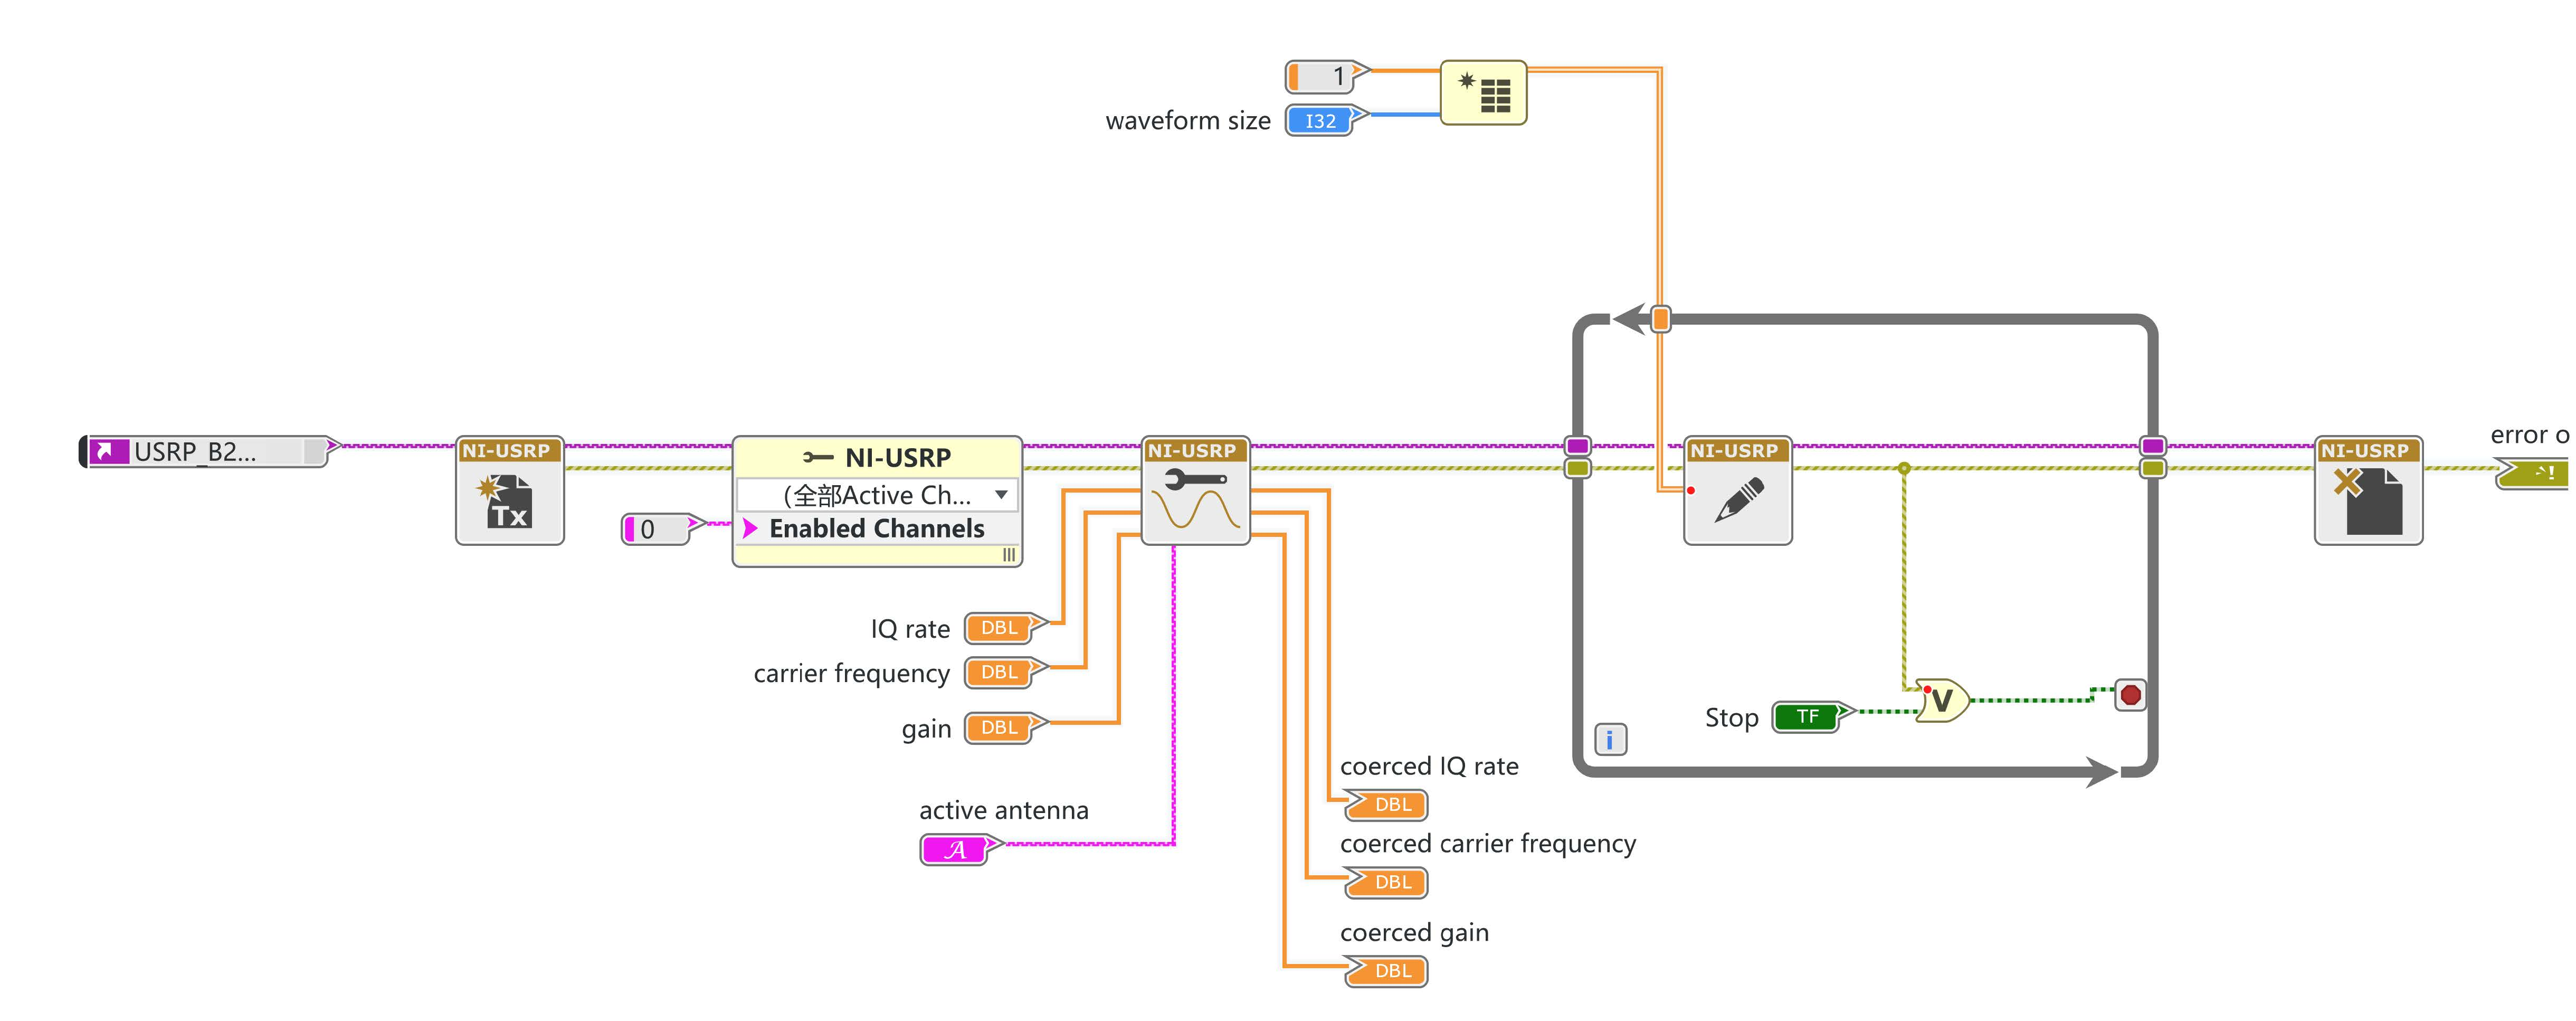
\includegraphics[width = 0.4\textwidth]{lab9/carrier.jpg}
    \caption{载波信号发送电路图}
\end{figure}
\begin{figure}[H]
    \centering
    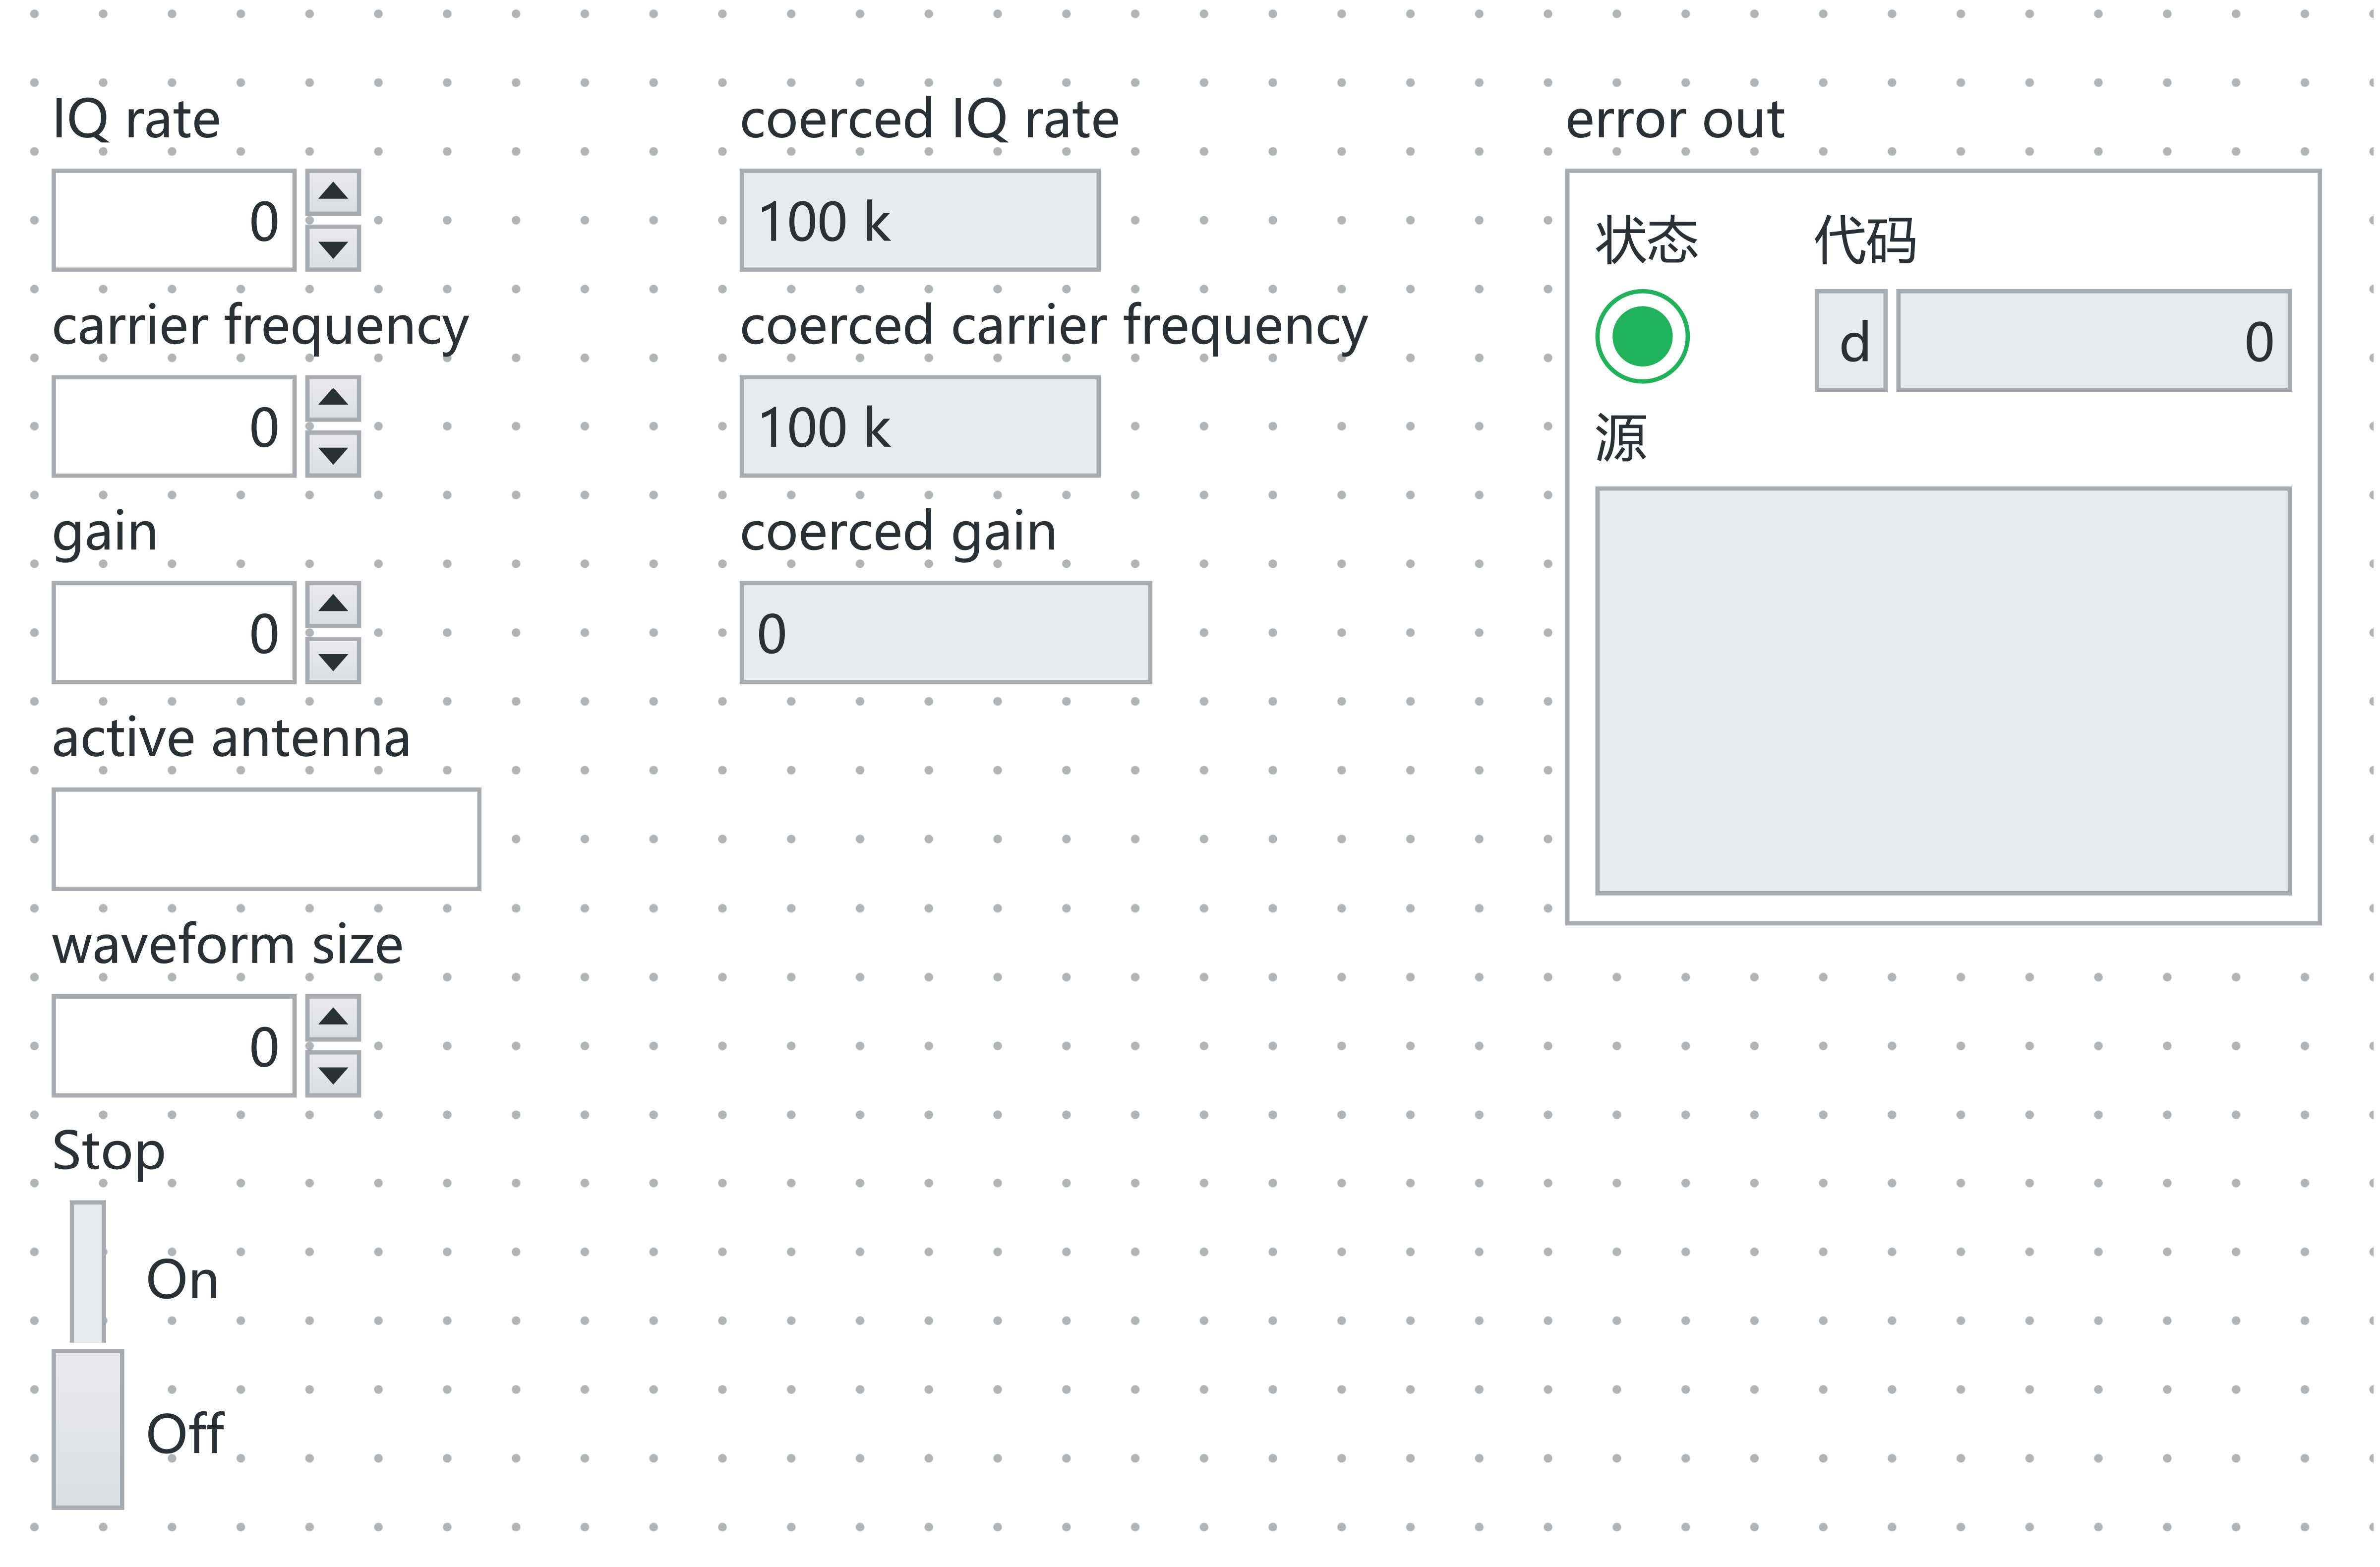
\includegraphics[width = 0.4\textwidth]{lab9/carrier-b.jpg}
    \caption{载波信号发送电路前面版图}
\end{figure}

设置好参数,运行电路,使用 SMA 电缆将 USRP 设备的 TX1 输出端口连接到频谱仪, 观察是否产生正确的信号频谱。

载波频率设置为2G,实际测试值为载波频率测出来为1.999994166GHz,考虑到有误差,符合实际情况。

改变载波信号频率值,取 1G、2.5G、3G、4G、5G、……,使用频谱仪确认频率是 否正确
\begin{figure}[H]
    \centering
    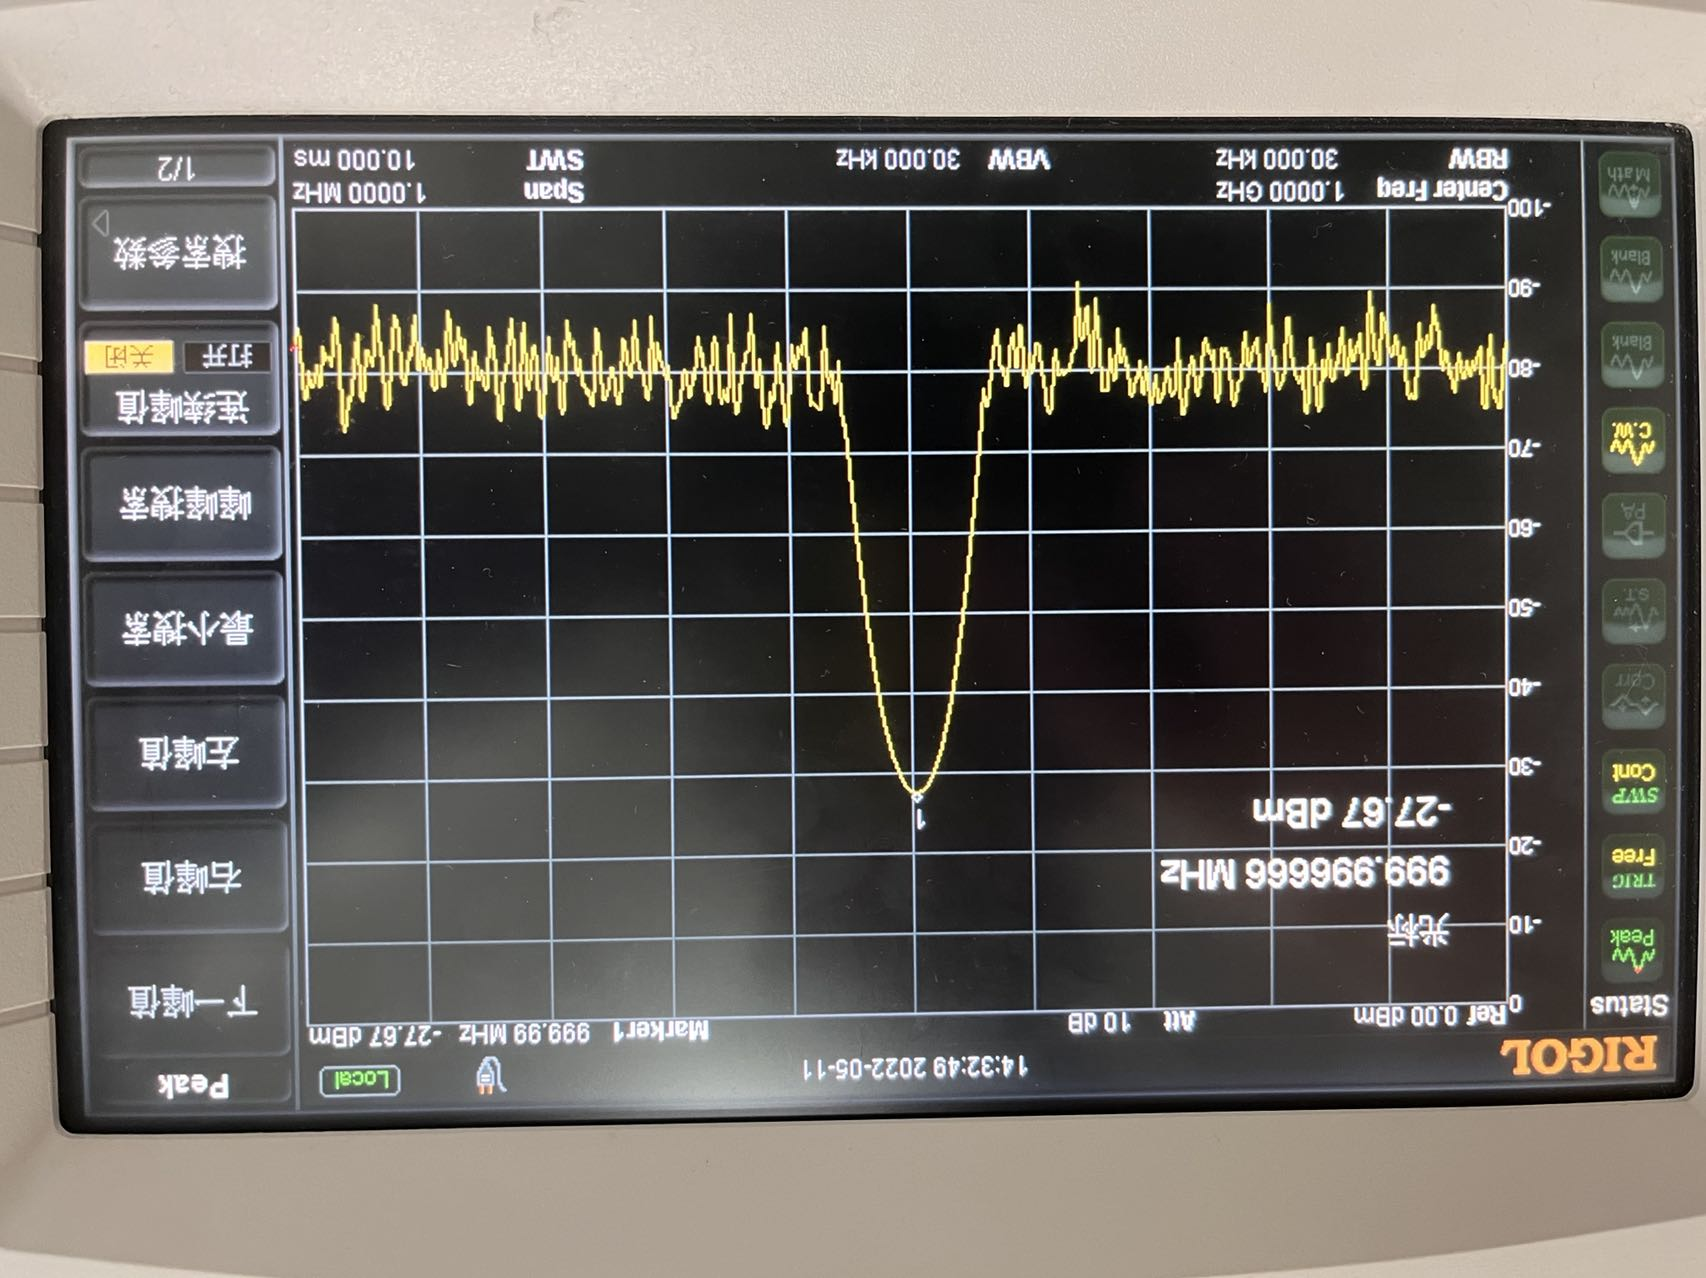
\includegraphics[width = 0.4\textwidth,angle=180]{lab9/1.jpg}
    \caption{载波频率为1G的频谱图}
\end{figure}

\begin{figure}[H]
    \centering
    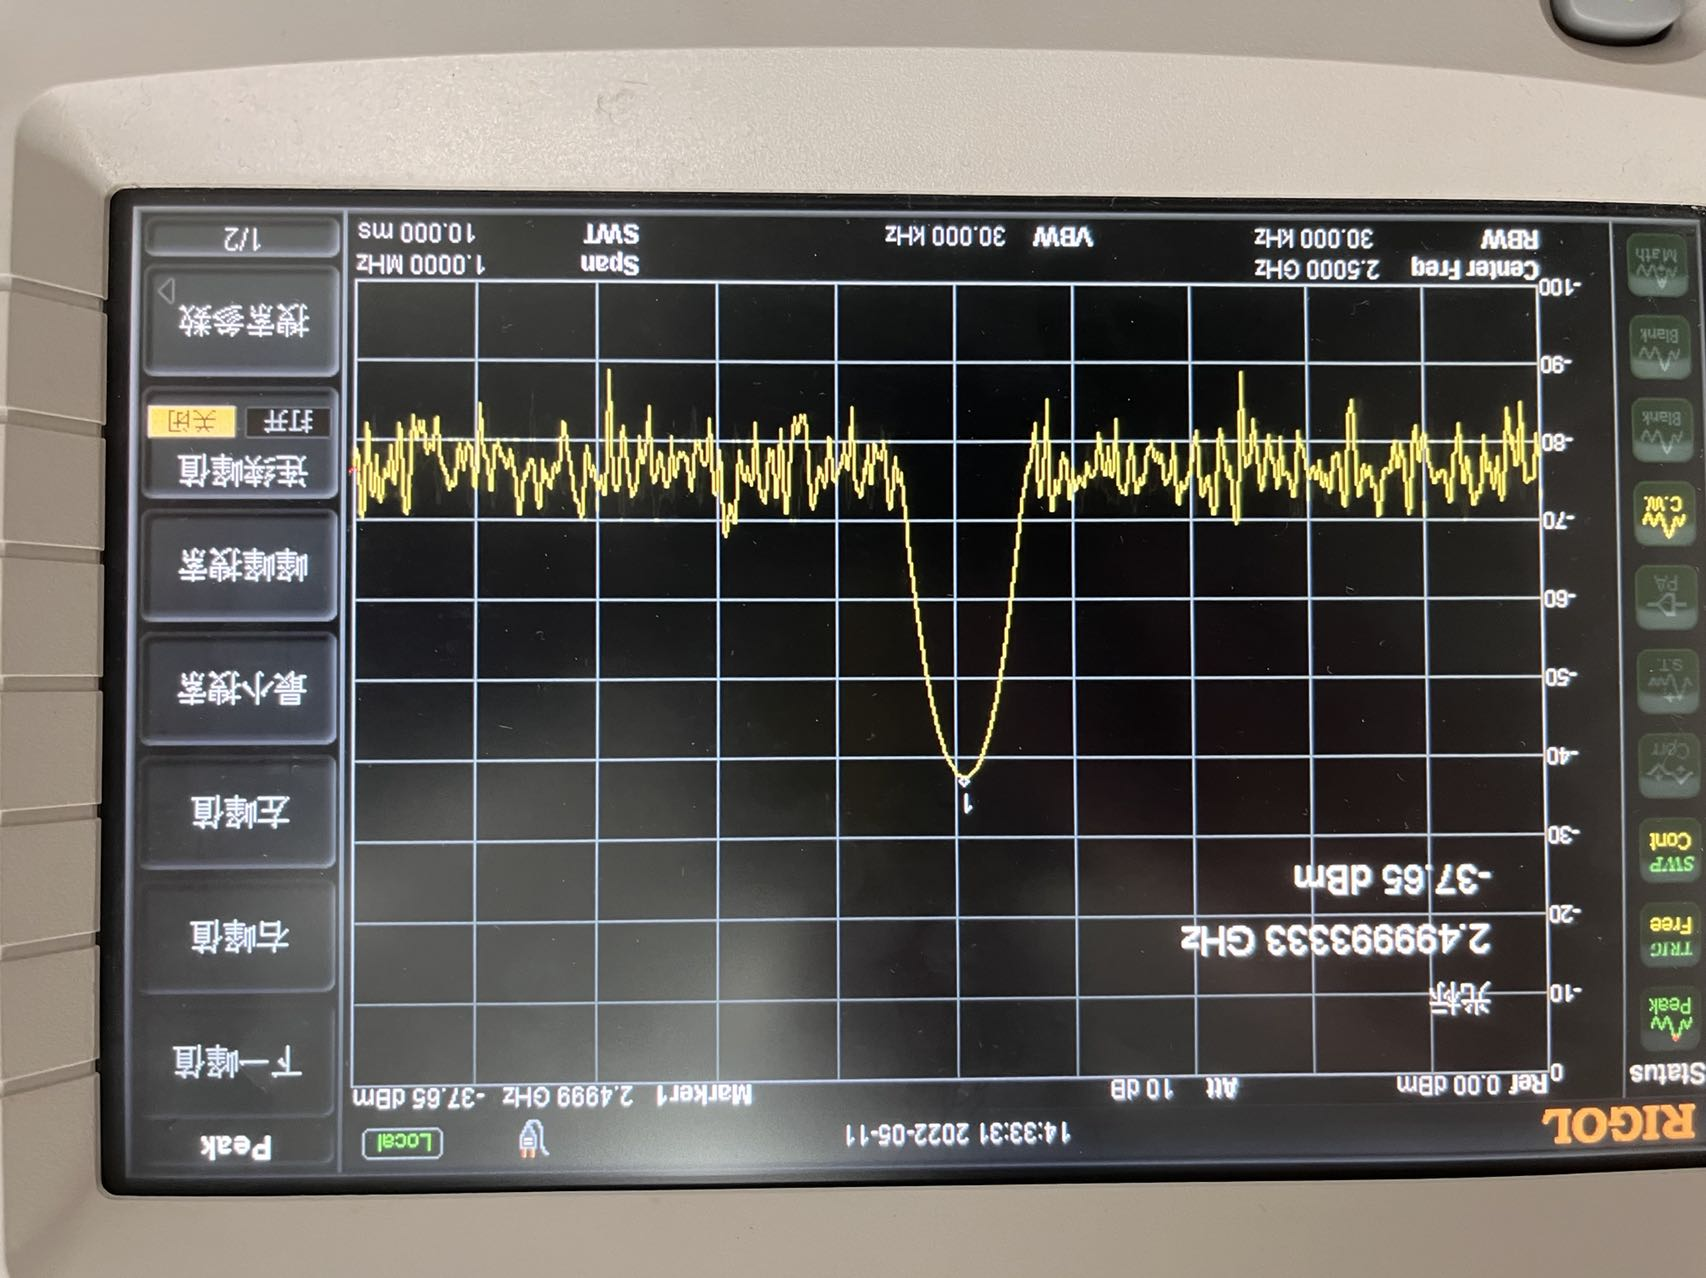
\includegraphics[width = 0.4\textwidth,angle=180]{lab9/2.jpg}
    \caption{载波频率为2.5G的频谱图}
\end{figure}
\begin{figure}[H]
    \centering
    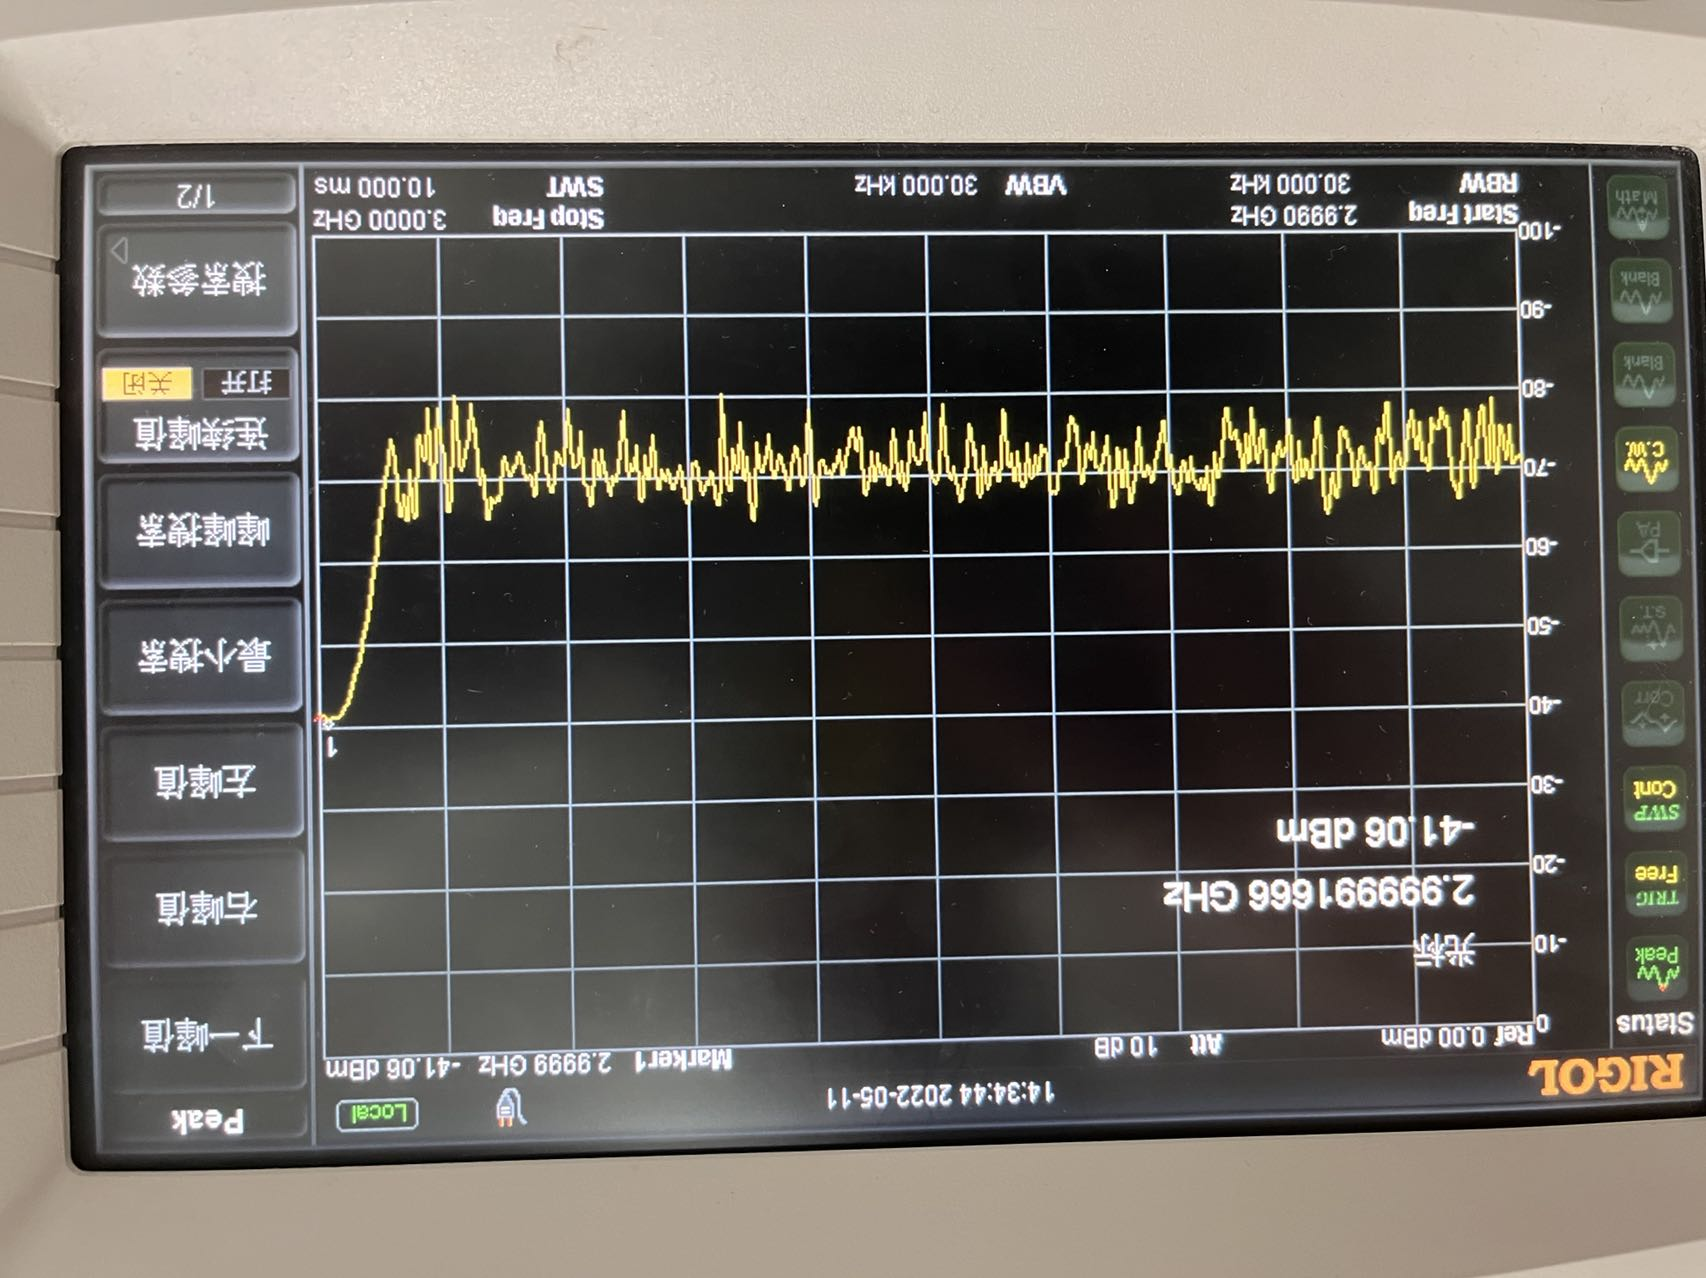
\includegraphics[width = 0.4\textwidth,angle=180]{lab9/3.jpg}
    \caption{载波频率为3G的频谱图}
\end{figure}

从上述的频谱图中可以看出,虽然与设置的载波频率有偏差,但仍然是正确的。但当设置的载波频率过大时,频谱仪将会显示不出来。

\subsubsection{单音信号上边带传输}
\begin{figure}[H]
    \centering
    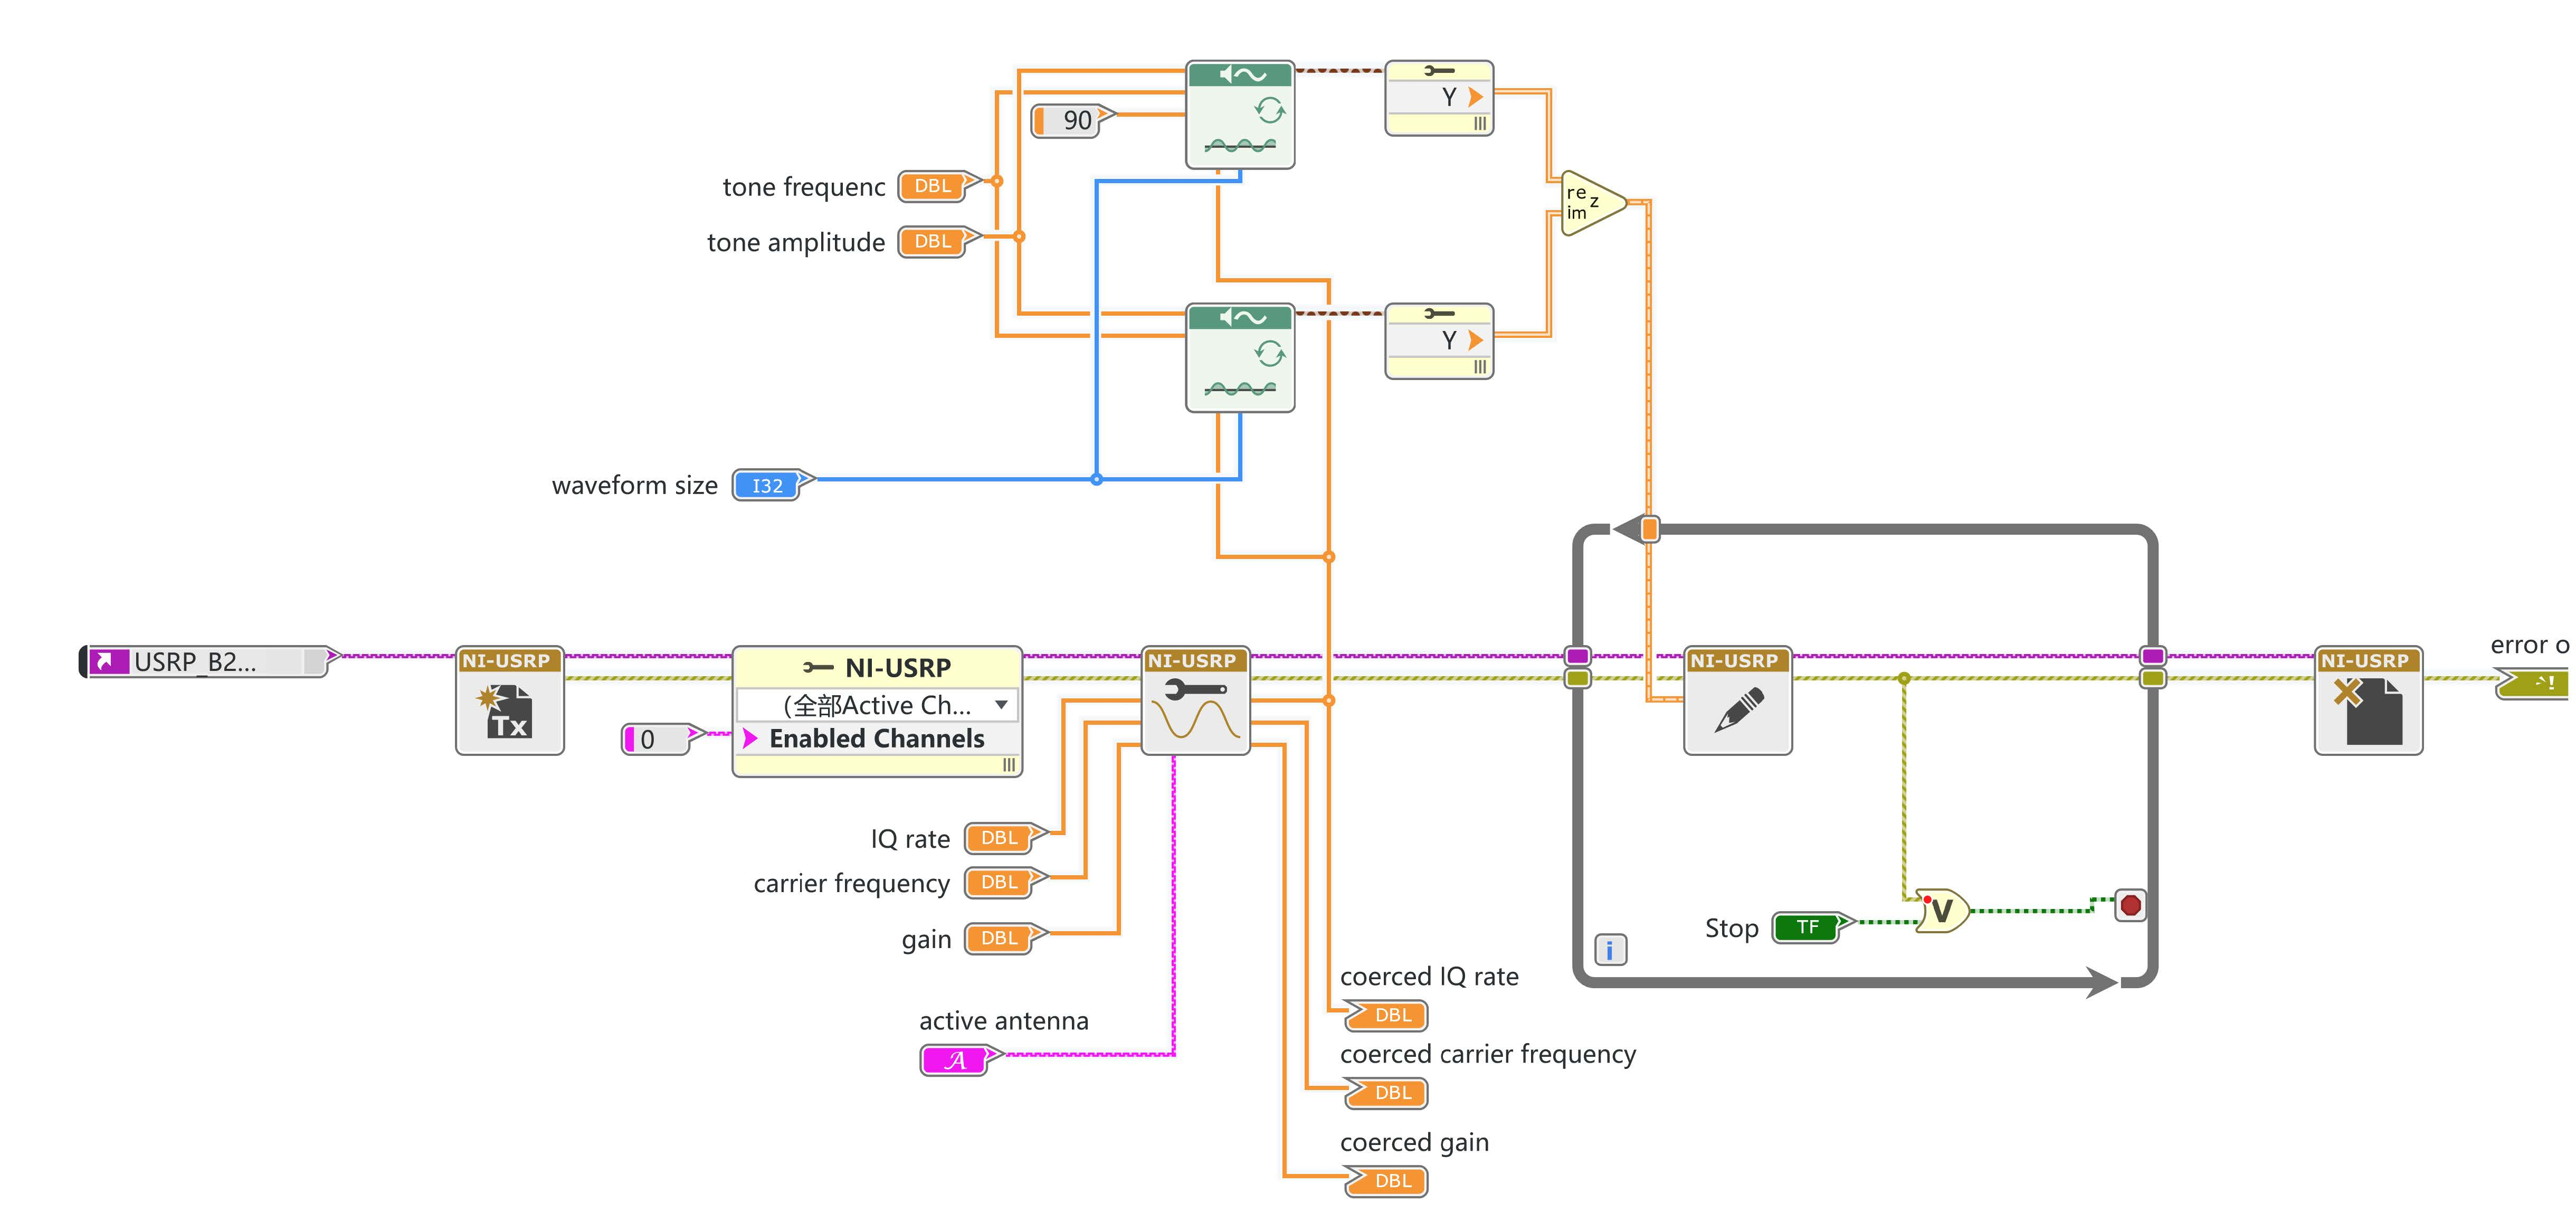
\includegraphics[width = 0.4\textwidth]{lab9/upper-side_IQ-a.jpg}
    \caption{上边带调制发送电路图}
\end{figure}
\begin{figure}[H]
    \centering
    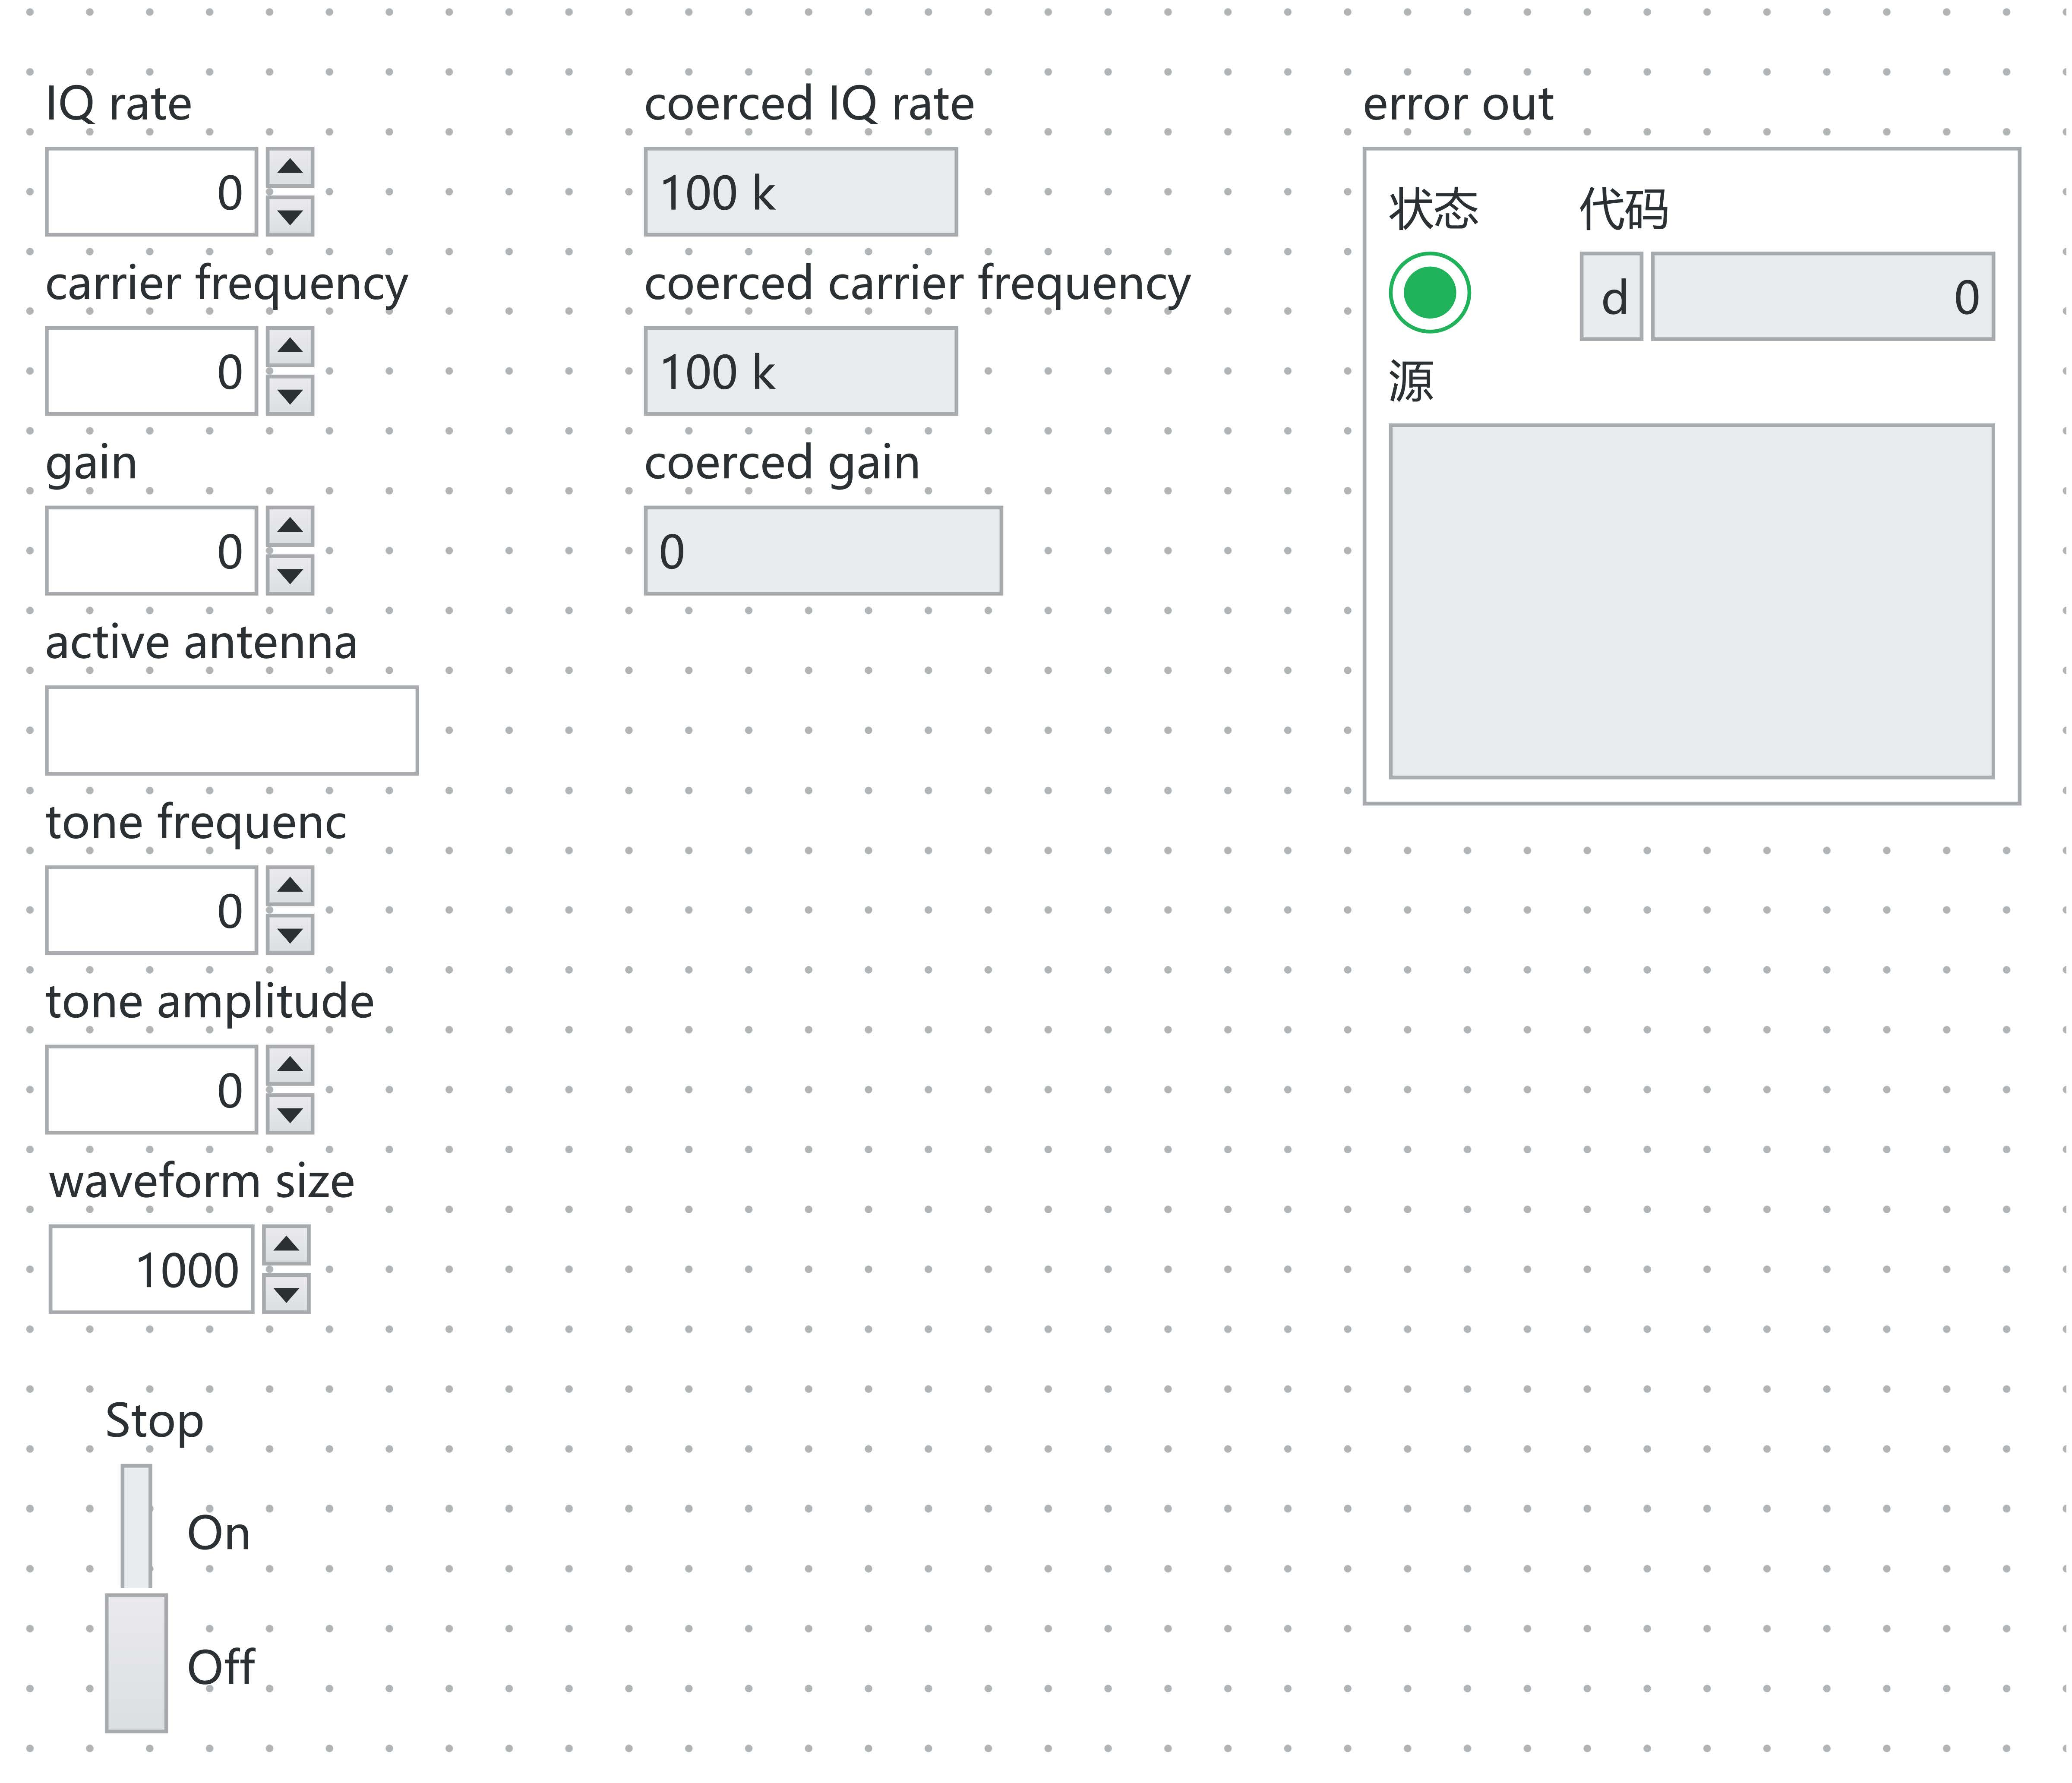
\includegraphics[width = 0.4\textwidth]{lab9/upper-side_IQ-b.jpg}
    \caption{上边带调制发送前面板图}
\end{figure}
设置好参数,运行电路,使用 SMA 电缆将 USRP 设备的 TX1 输出端口连接到频谱仪, 观察是否产生正确的信号频谱。
\begin{figure}[H]
    \centering
    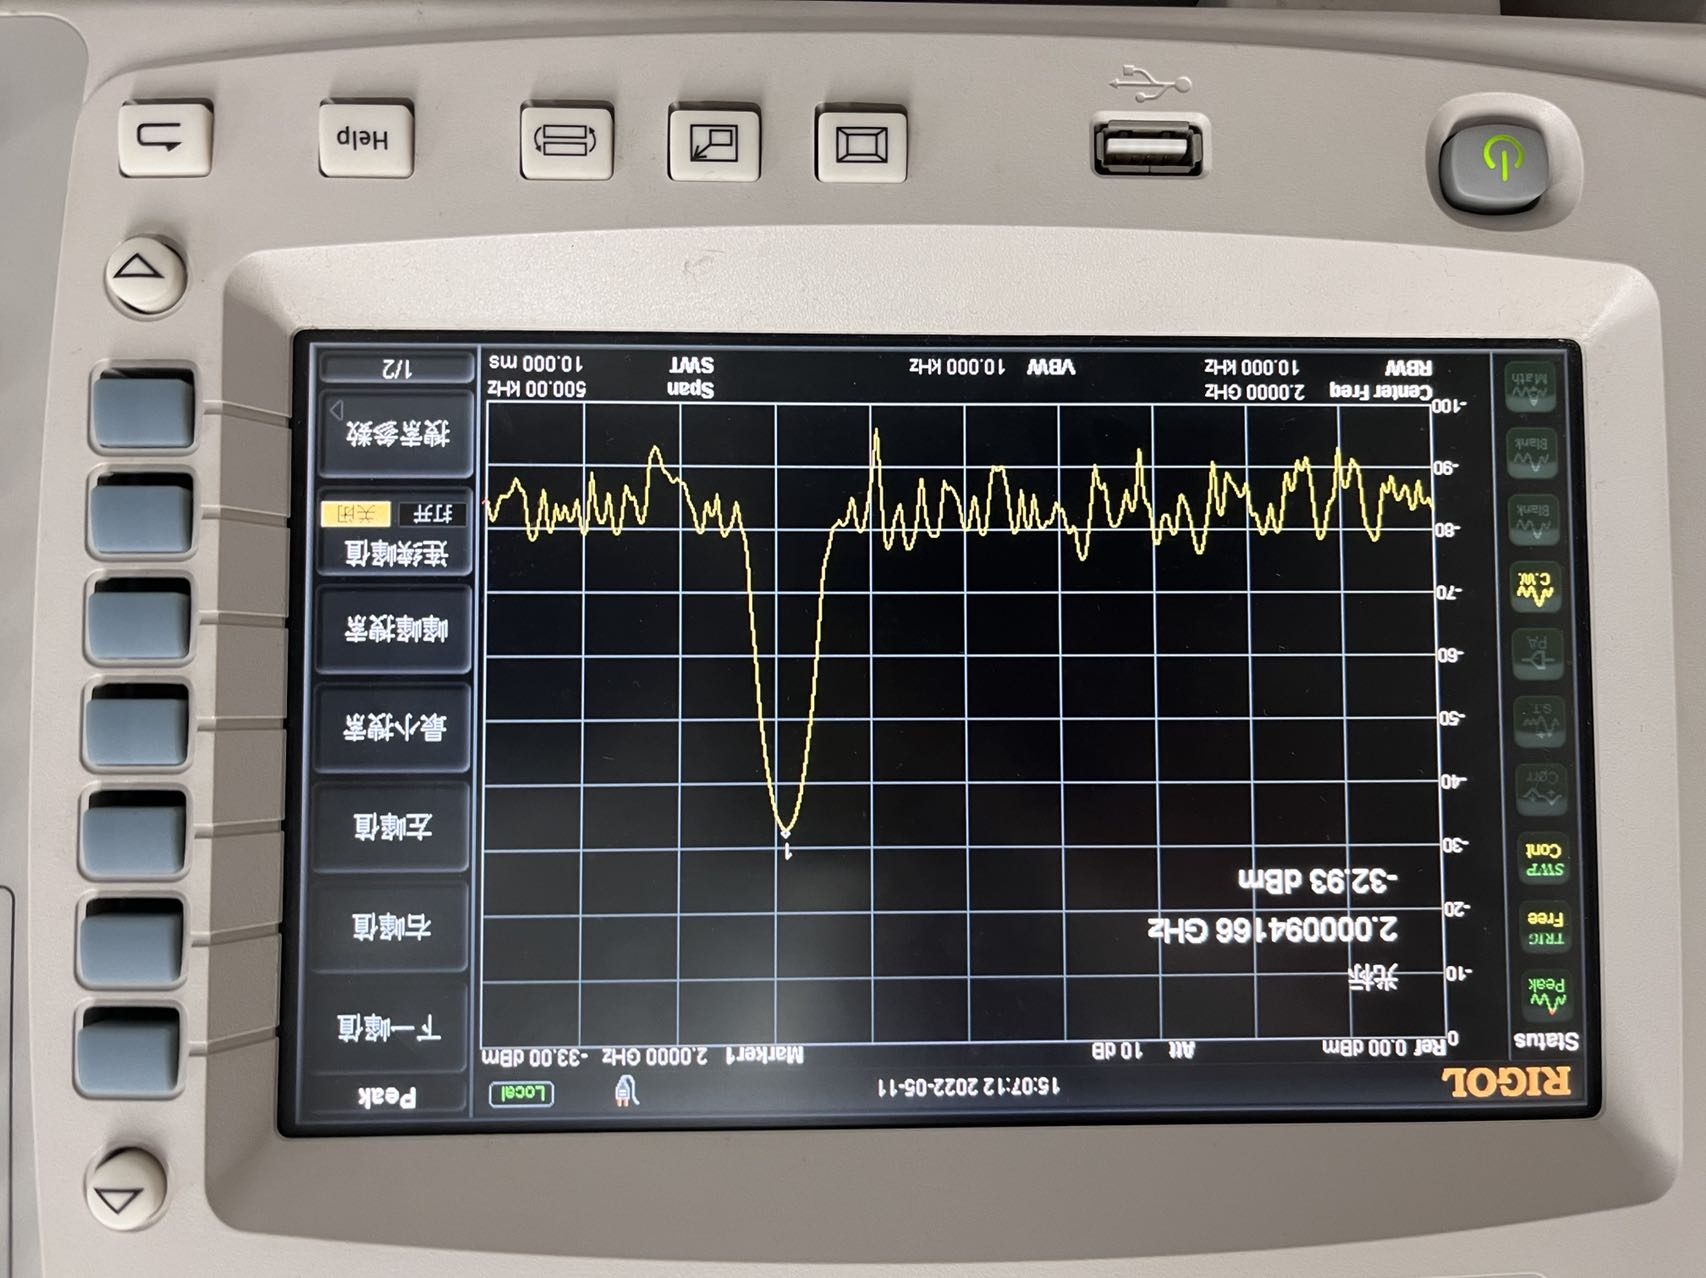
\includegraphics[width = 0.4\textwidth,angle=180]{lab9/5.jpg}
    \caption{上边带调制信号频谱图示例}
\end{figure}

改变 tone frequency 的值,分别取:10k、50k、100k,用频谱分析仪观察上边带 信号的频谱变化。
\begin{table}[H]
    \centering
    \begin{tabular}{|l|l|l|}
        \hline
        \textbf{tone frequency} & \textbf{上边带信号频谱中心频率} \\ \hline
        \textbf{1kHz}           & \textbf{1.999995166GHz}         \\ \hline
        \textbf{10kHz}          & \textbf{2.000004166GHz}         \\ \hline
        \textbf{50kHz}          & \textbf{2.000044166GHz}         \\ \hline
        \textbf{100kHz}         & \textbf{2.000094166GHz}         \\ \hline
    \end{tabular}
\end{table}

载波频率测出来为1.999994166GHz显然上边带信号的中心频率为载波频率加上tone frequency。
\subsection{问题 1}
(1) 在相同载波频率情况下,比较载波发生电路和上变频电路的信号频谱。

显然,相对于载波频率的峰值,上变频电路的频谱峰值对应的频率高$\omega_0$,此$\omega_0$即为tone frequency.

(2) 改变 waveform size 参数至 1005,观察信号的频谱。

\begin{figure}[H]
    \centering
    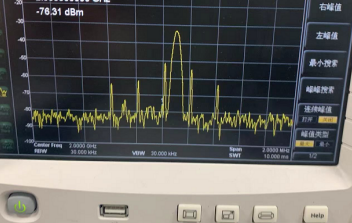
\includegraphics[width = 0.25\textwidth]{lab9/wave.png}
    \caption{waveform=1005}
\end{figure}
出现了一些其他频谱的脉冲,可能是由于频谱泄露带来的问题。

(3) 新建一个“lower-side\_IQ.gvi”,完成下变频电路,观察信号的频谱

电路设计上在上边带的基础上,只要将相位改变180度,将相加变为相减,具体过程为:

$\cos \omega t \times \cos \omega_{0} t-\sin \omega t \times \sin \omega_{0} t$
$=\frac{1}{2}\left[\cos \left(\omega+\omega_{0}\right) t+\cos \left(\omega-\omega_{0}\right) t\right]-\frac{1}{2}\left[\cos \left(\omega+\omega_{0}\right) t-\cos \left(\omega-\omega_{0}\right) t\right]$
$=\cos \left(\omega-\omega_{0}\right) t$
便成了下边带。
\begin{figure}[H]
    \centering
    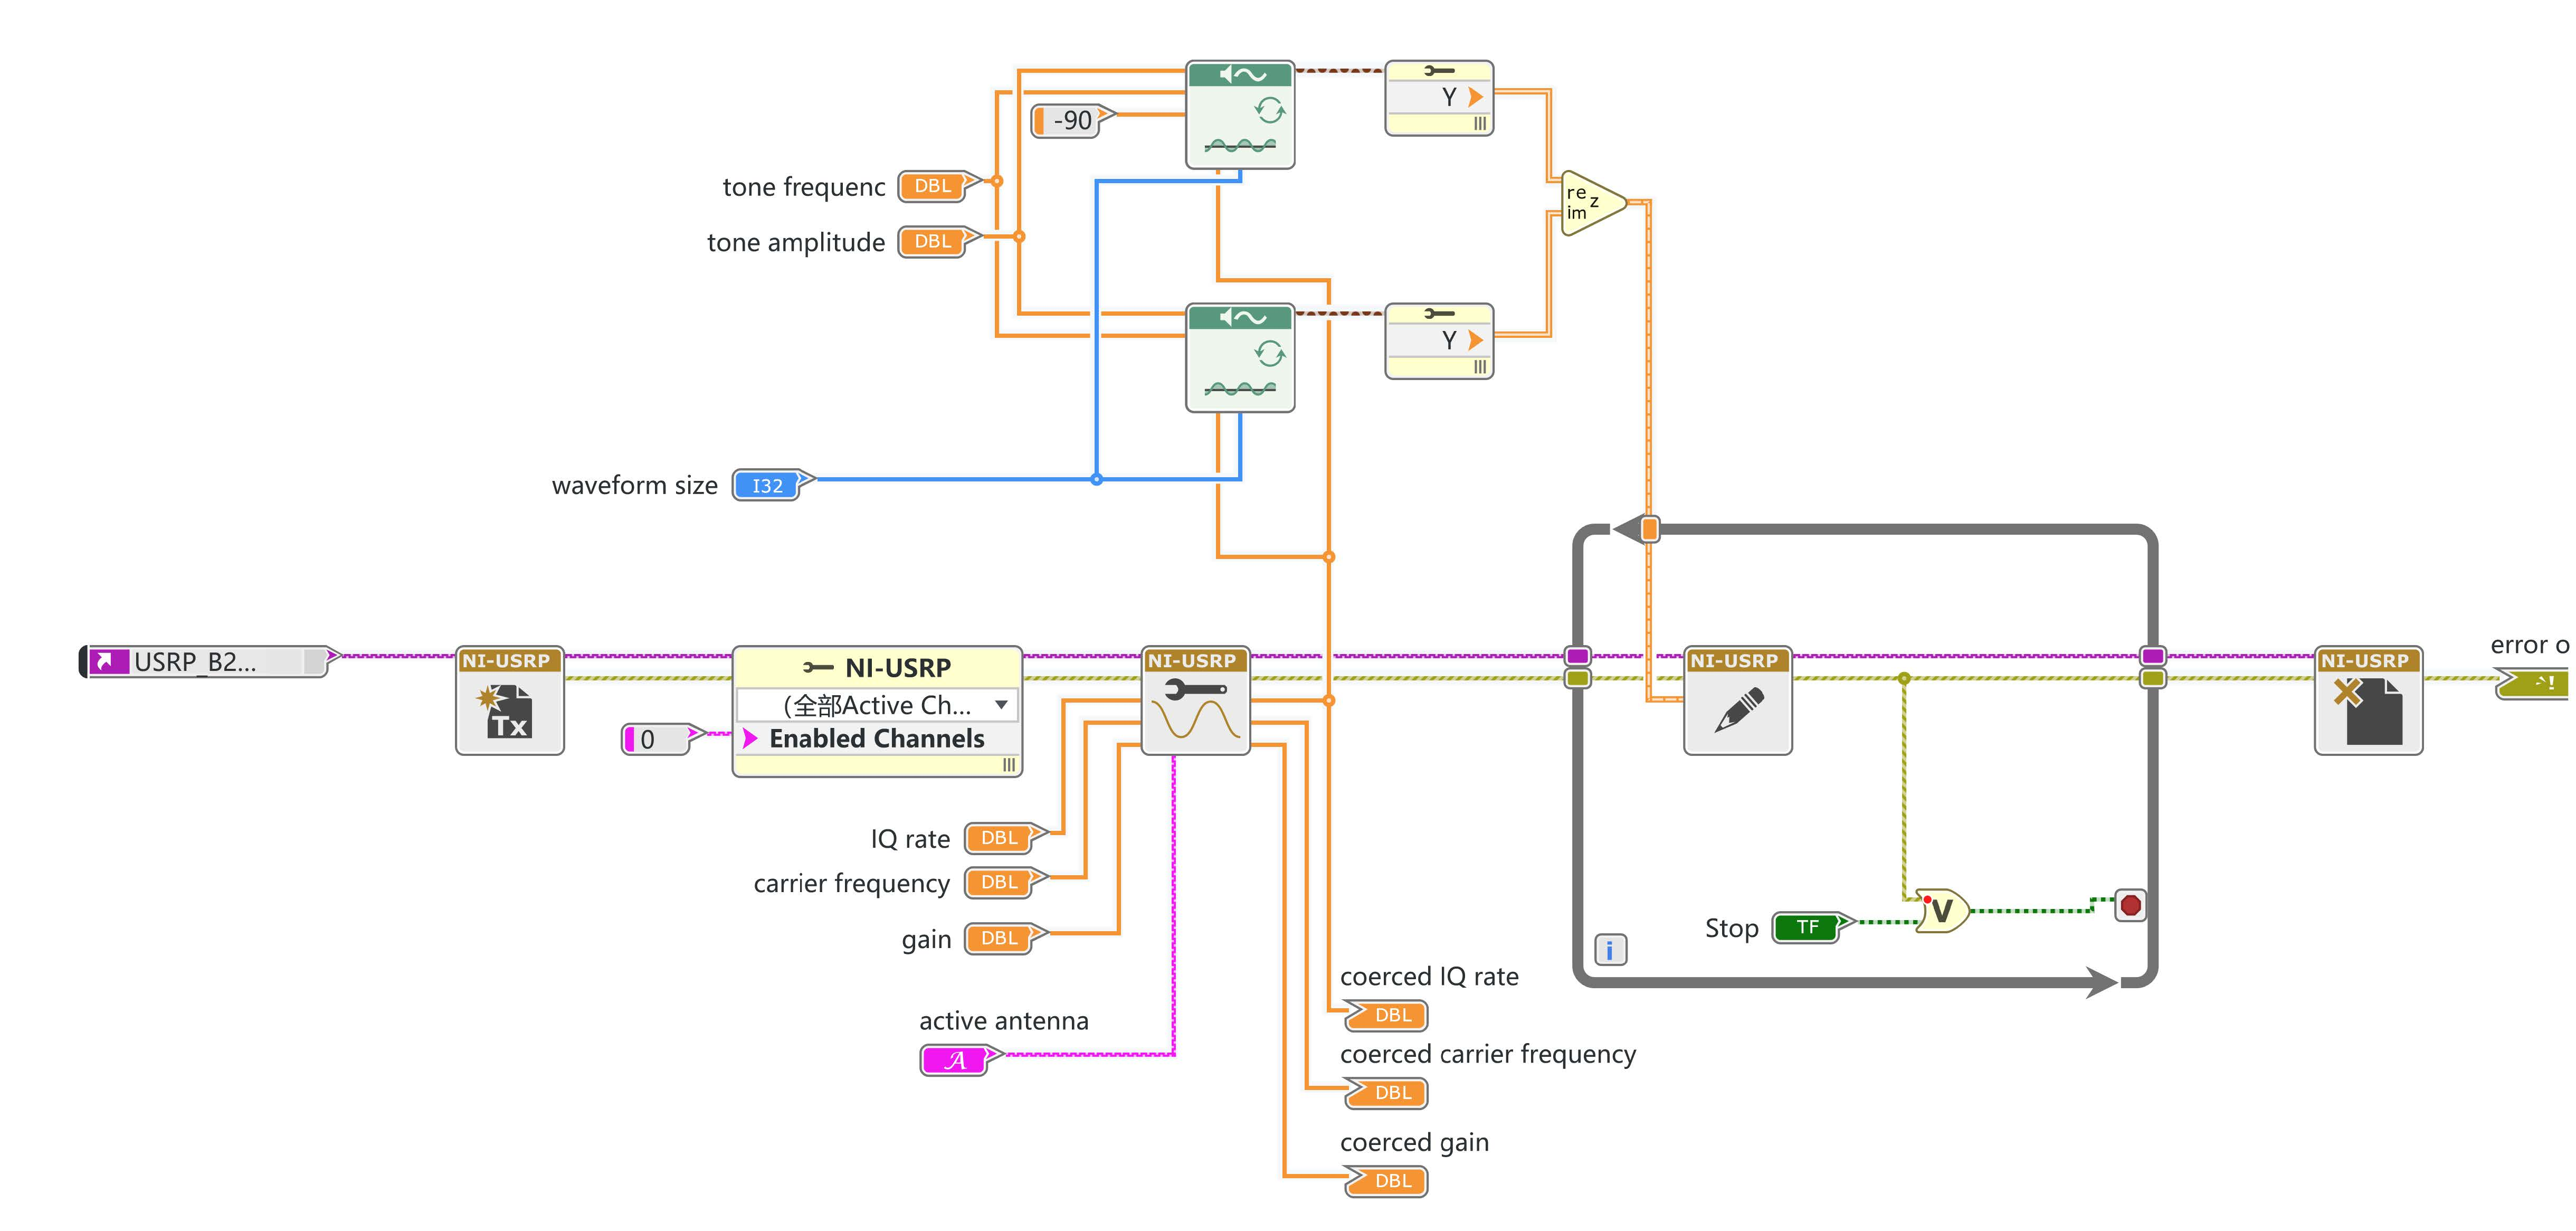
\includegraphics[width = 0.4\textwidth]{lab9/lower-side_IQ-a.jpg}
    \caption{下边带调制发送电路图}
\end{figure}
\begin{figure}[H]
    \centering
    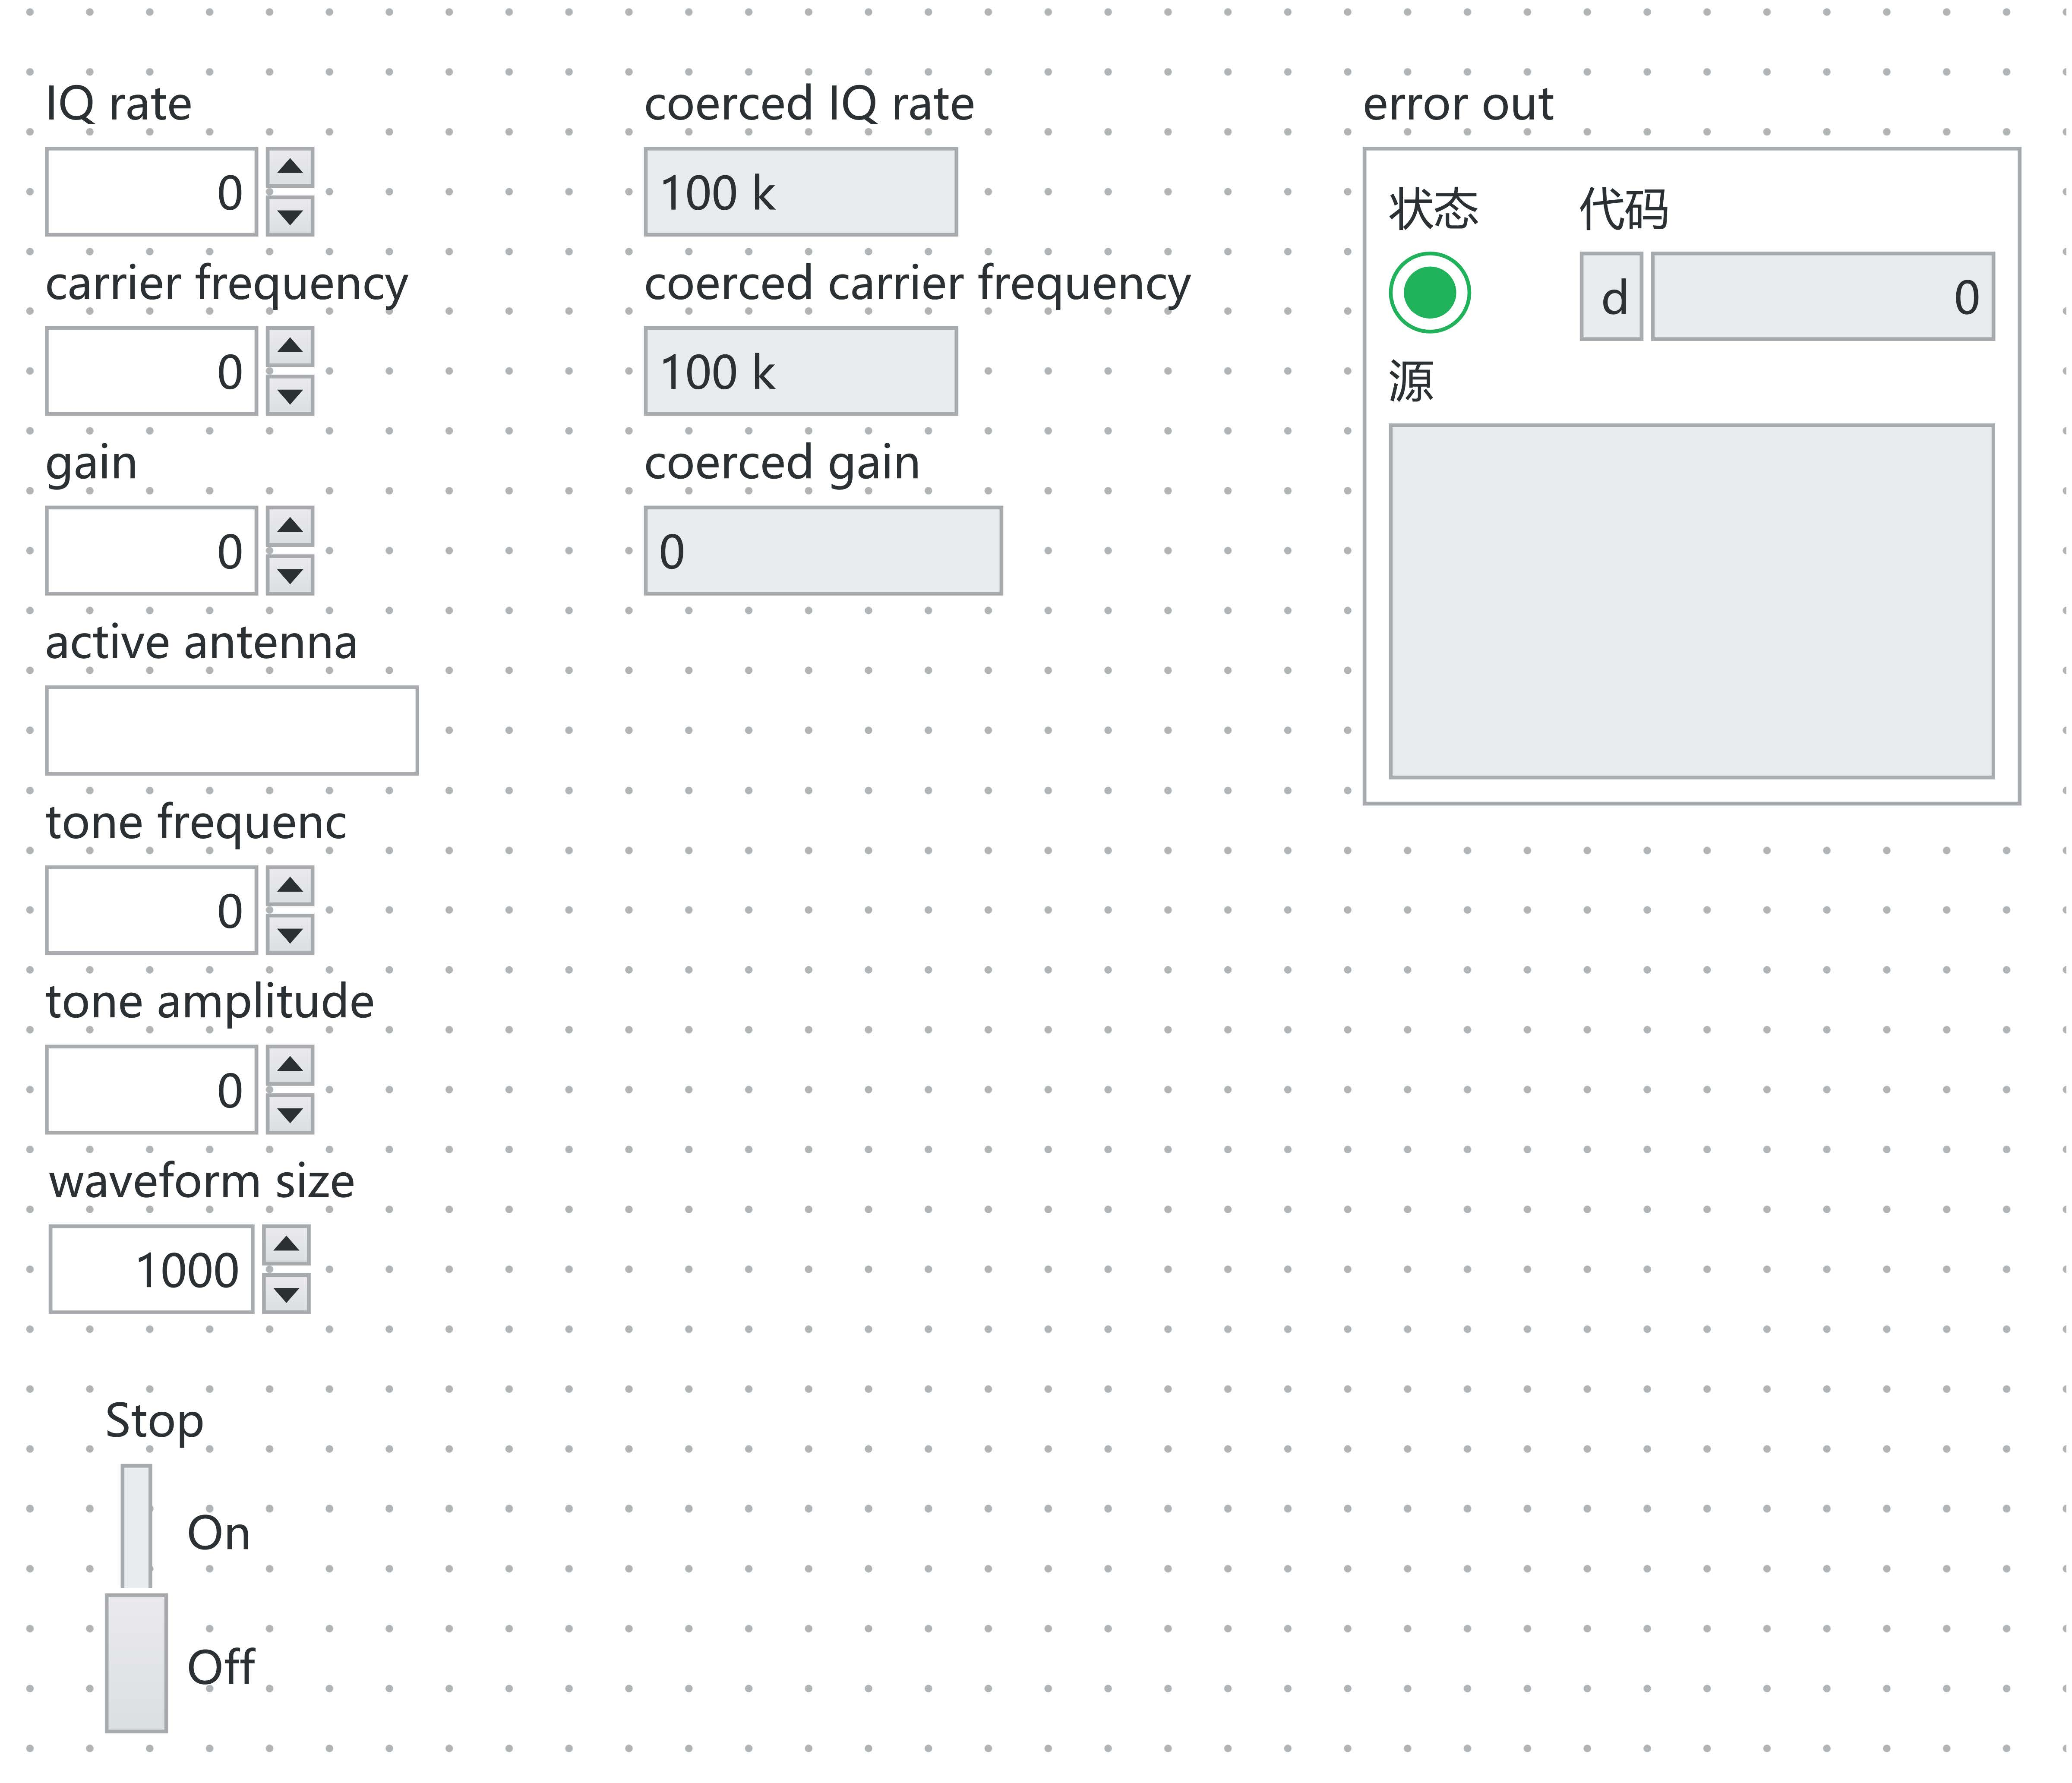
\includegraphics[width = 0.4\textwidth]{lab9/lower-side_IQ-b.jpg}
    \caption{下边带调制前面板图}
\end{figure}

\begin{figure}[H]
    \centering
    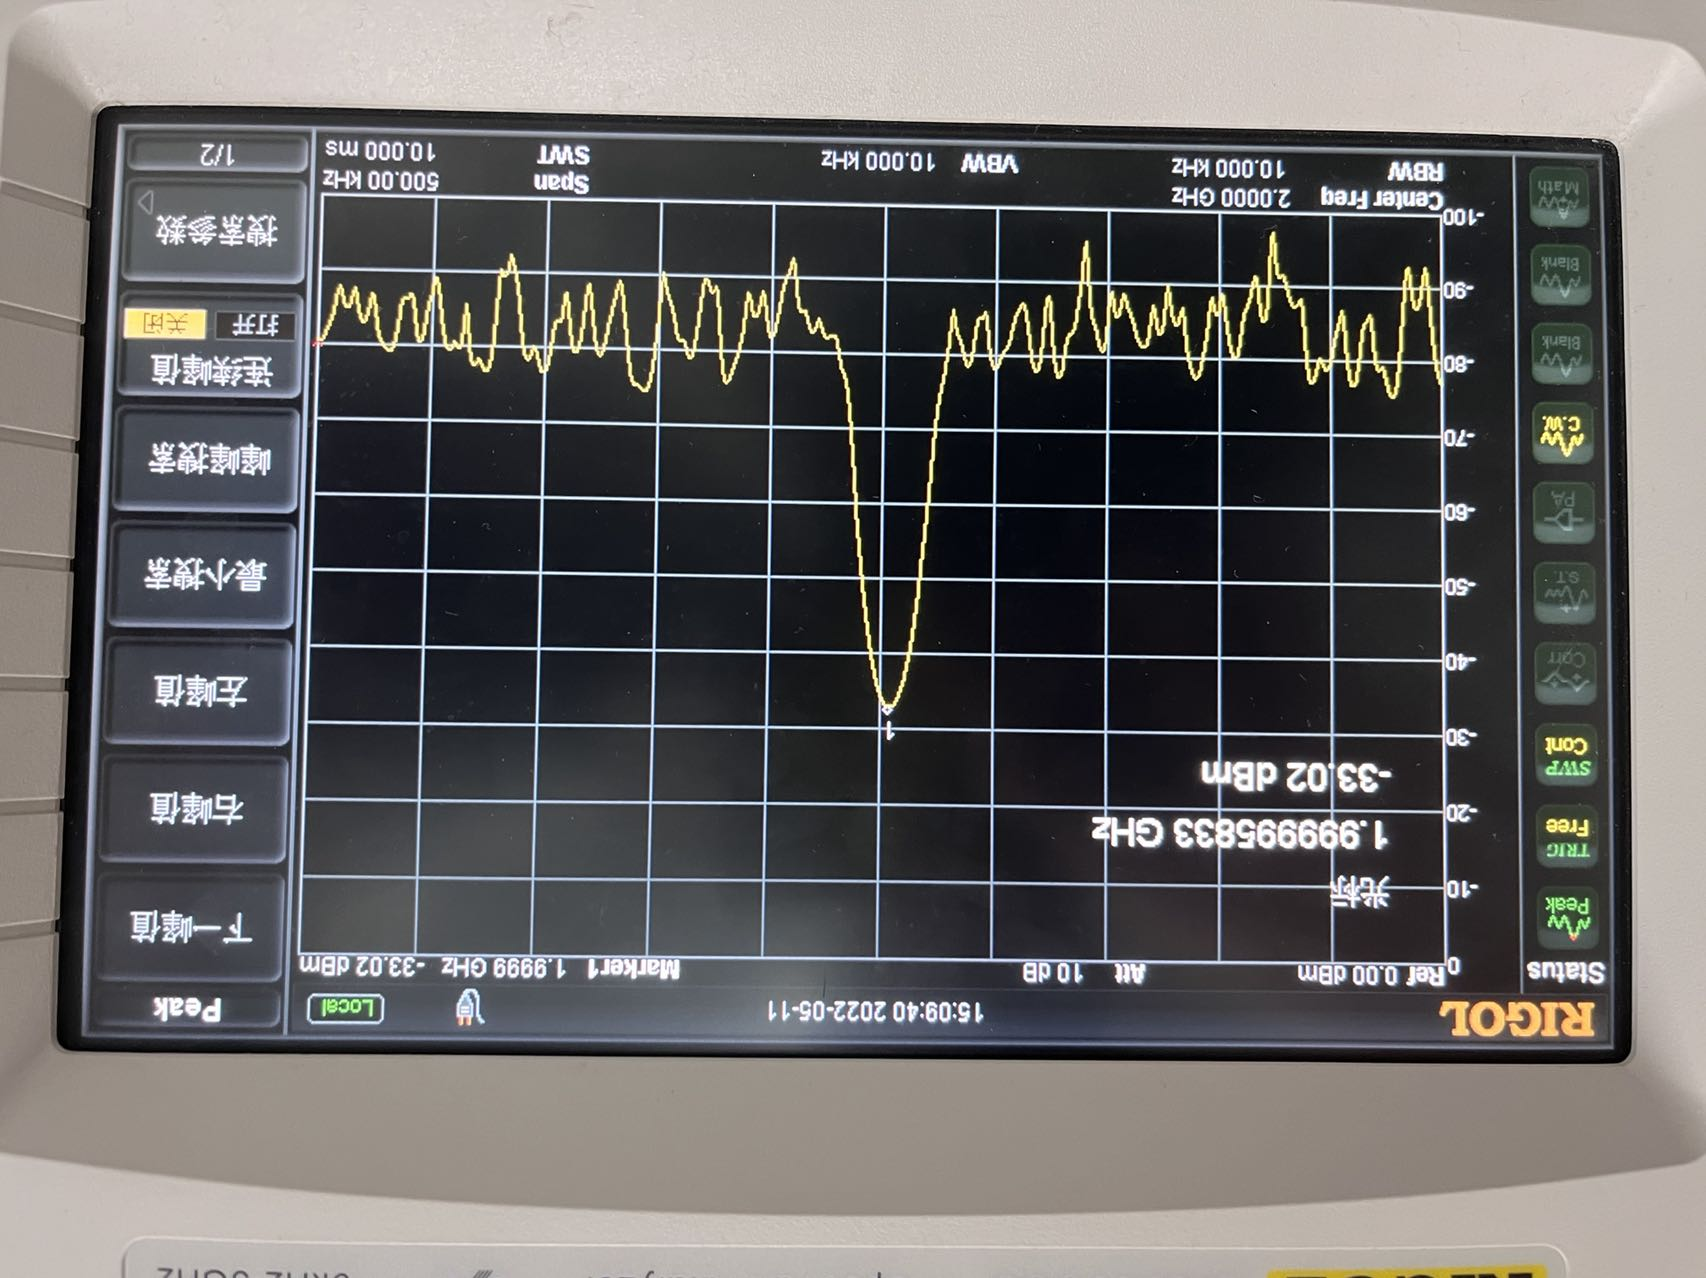
\includegraphics[width = 0.4\textwidth,angle=180]{lab9/6.jpg}
    \caption{下边带调制信号频谱图示例}
\end{figure}
显然,相对于载波频率的峰值,下边带调制的频谱峰值对应的频率低$\omega_0$,此$\omega_0$即为tone frequency.


(4) 新建一个“double-side\_IQ.gvi”,完成双边带电路,观察信号的频谱
电路设计上在上边带的基础上,只要将相位改成0度,相加的两边都有两个边带,相当于双边带的幅度变成原来的两倍,具体过程为:

$\cos \omega t \times \cos \omega_{0} t-\sin \omega t \times \sin \omega_{0} t$
$=\frac{1}{2}\left[\cos \left(\omega+\omega_{0}\right) t+\cos \left(\omega-\omega_{0}\right) t\right]+\frac{1}{2}\left[\cos \left(\omega+\omega_{0}\right) t+\cos \left(\omega-\omega_{0}\right) t\right]$
$=\cos \left(\omega+\omega_{0}\right) t+\cos \left(\omega-\omega_{0}\right) t$
便成了双边带。

\begin{figure}[H]
    \centering
    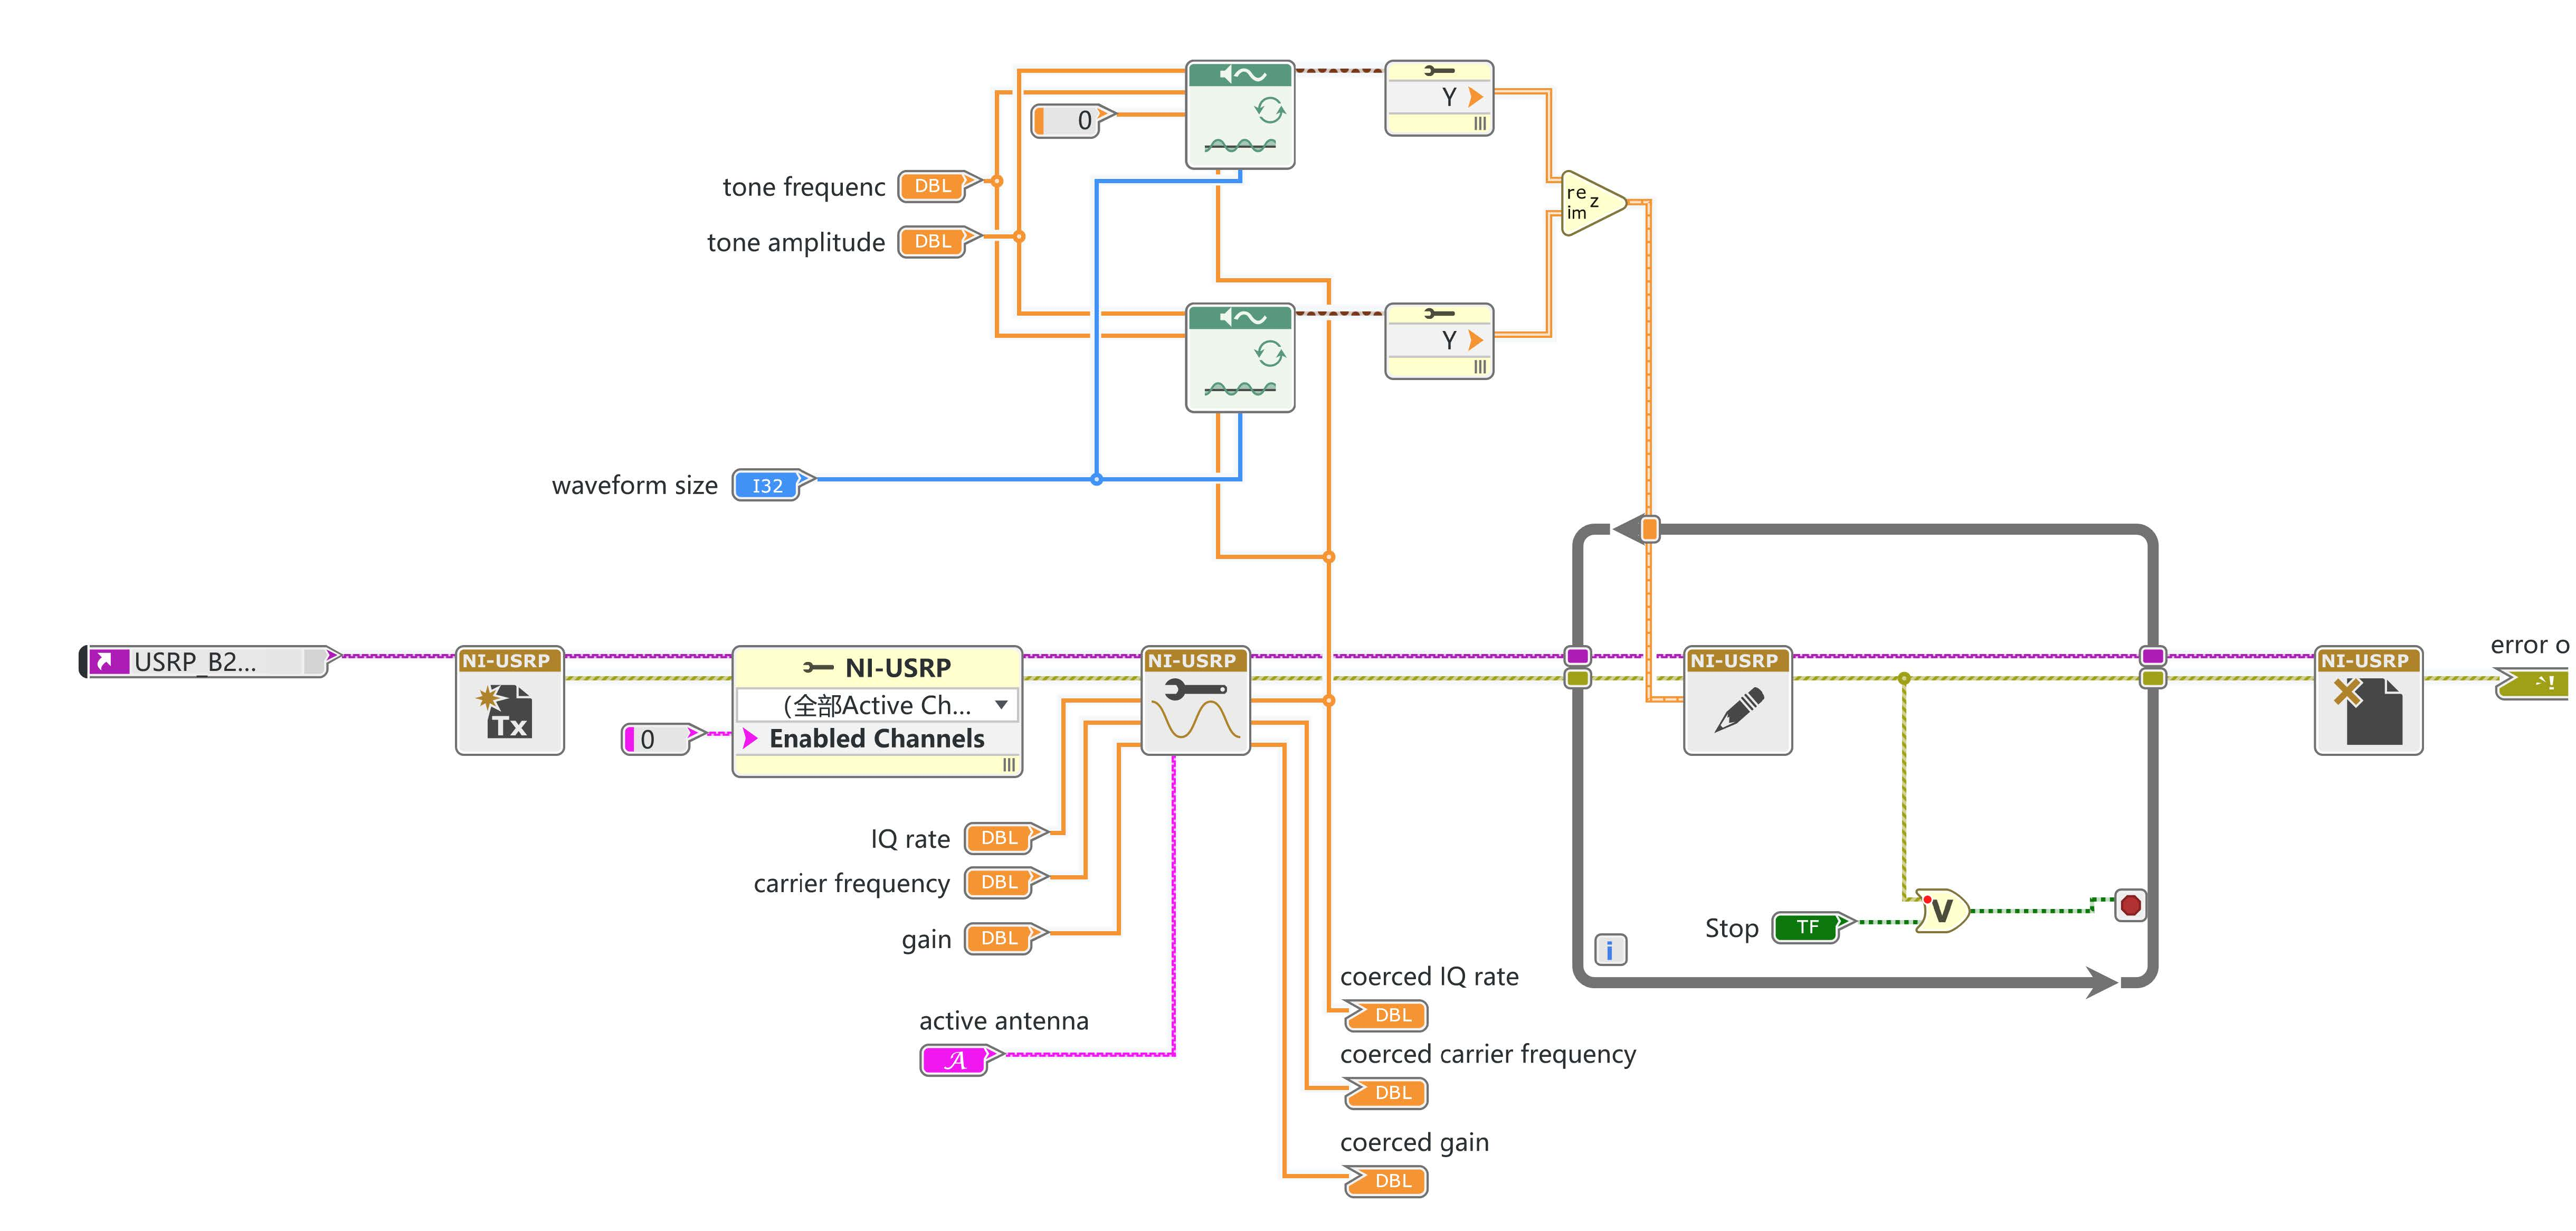
\includegraphics[width = 0.4\textwidth]{lab9/double-side_IQ-a.jpg}
    \caption{双边带调制发送电路图}
\end{figure}
\begin{figure}[H]
    \centering
    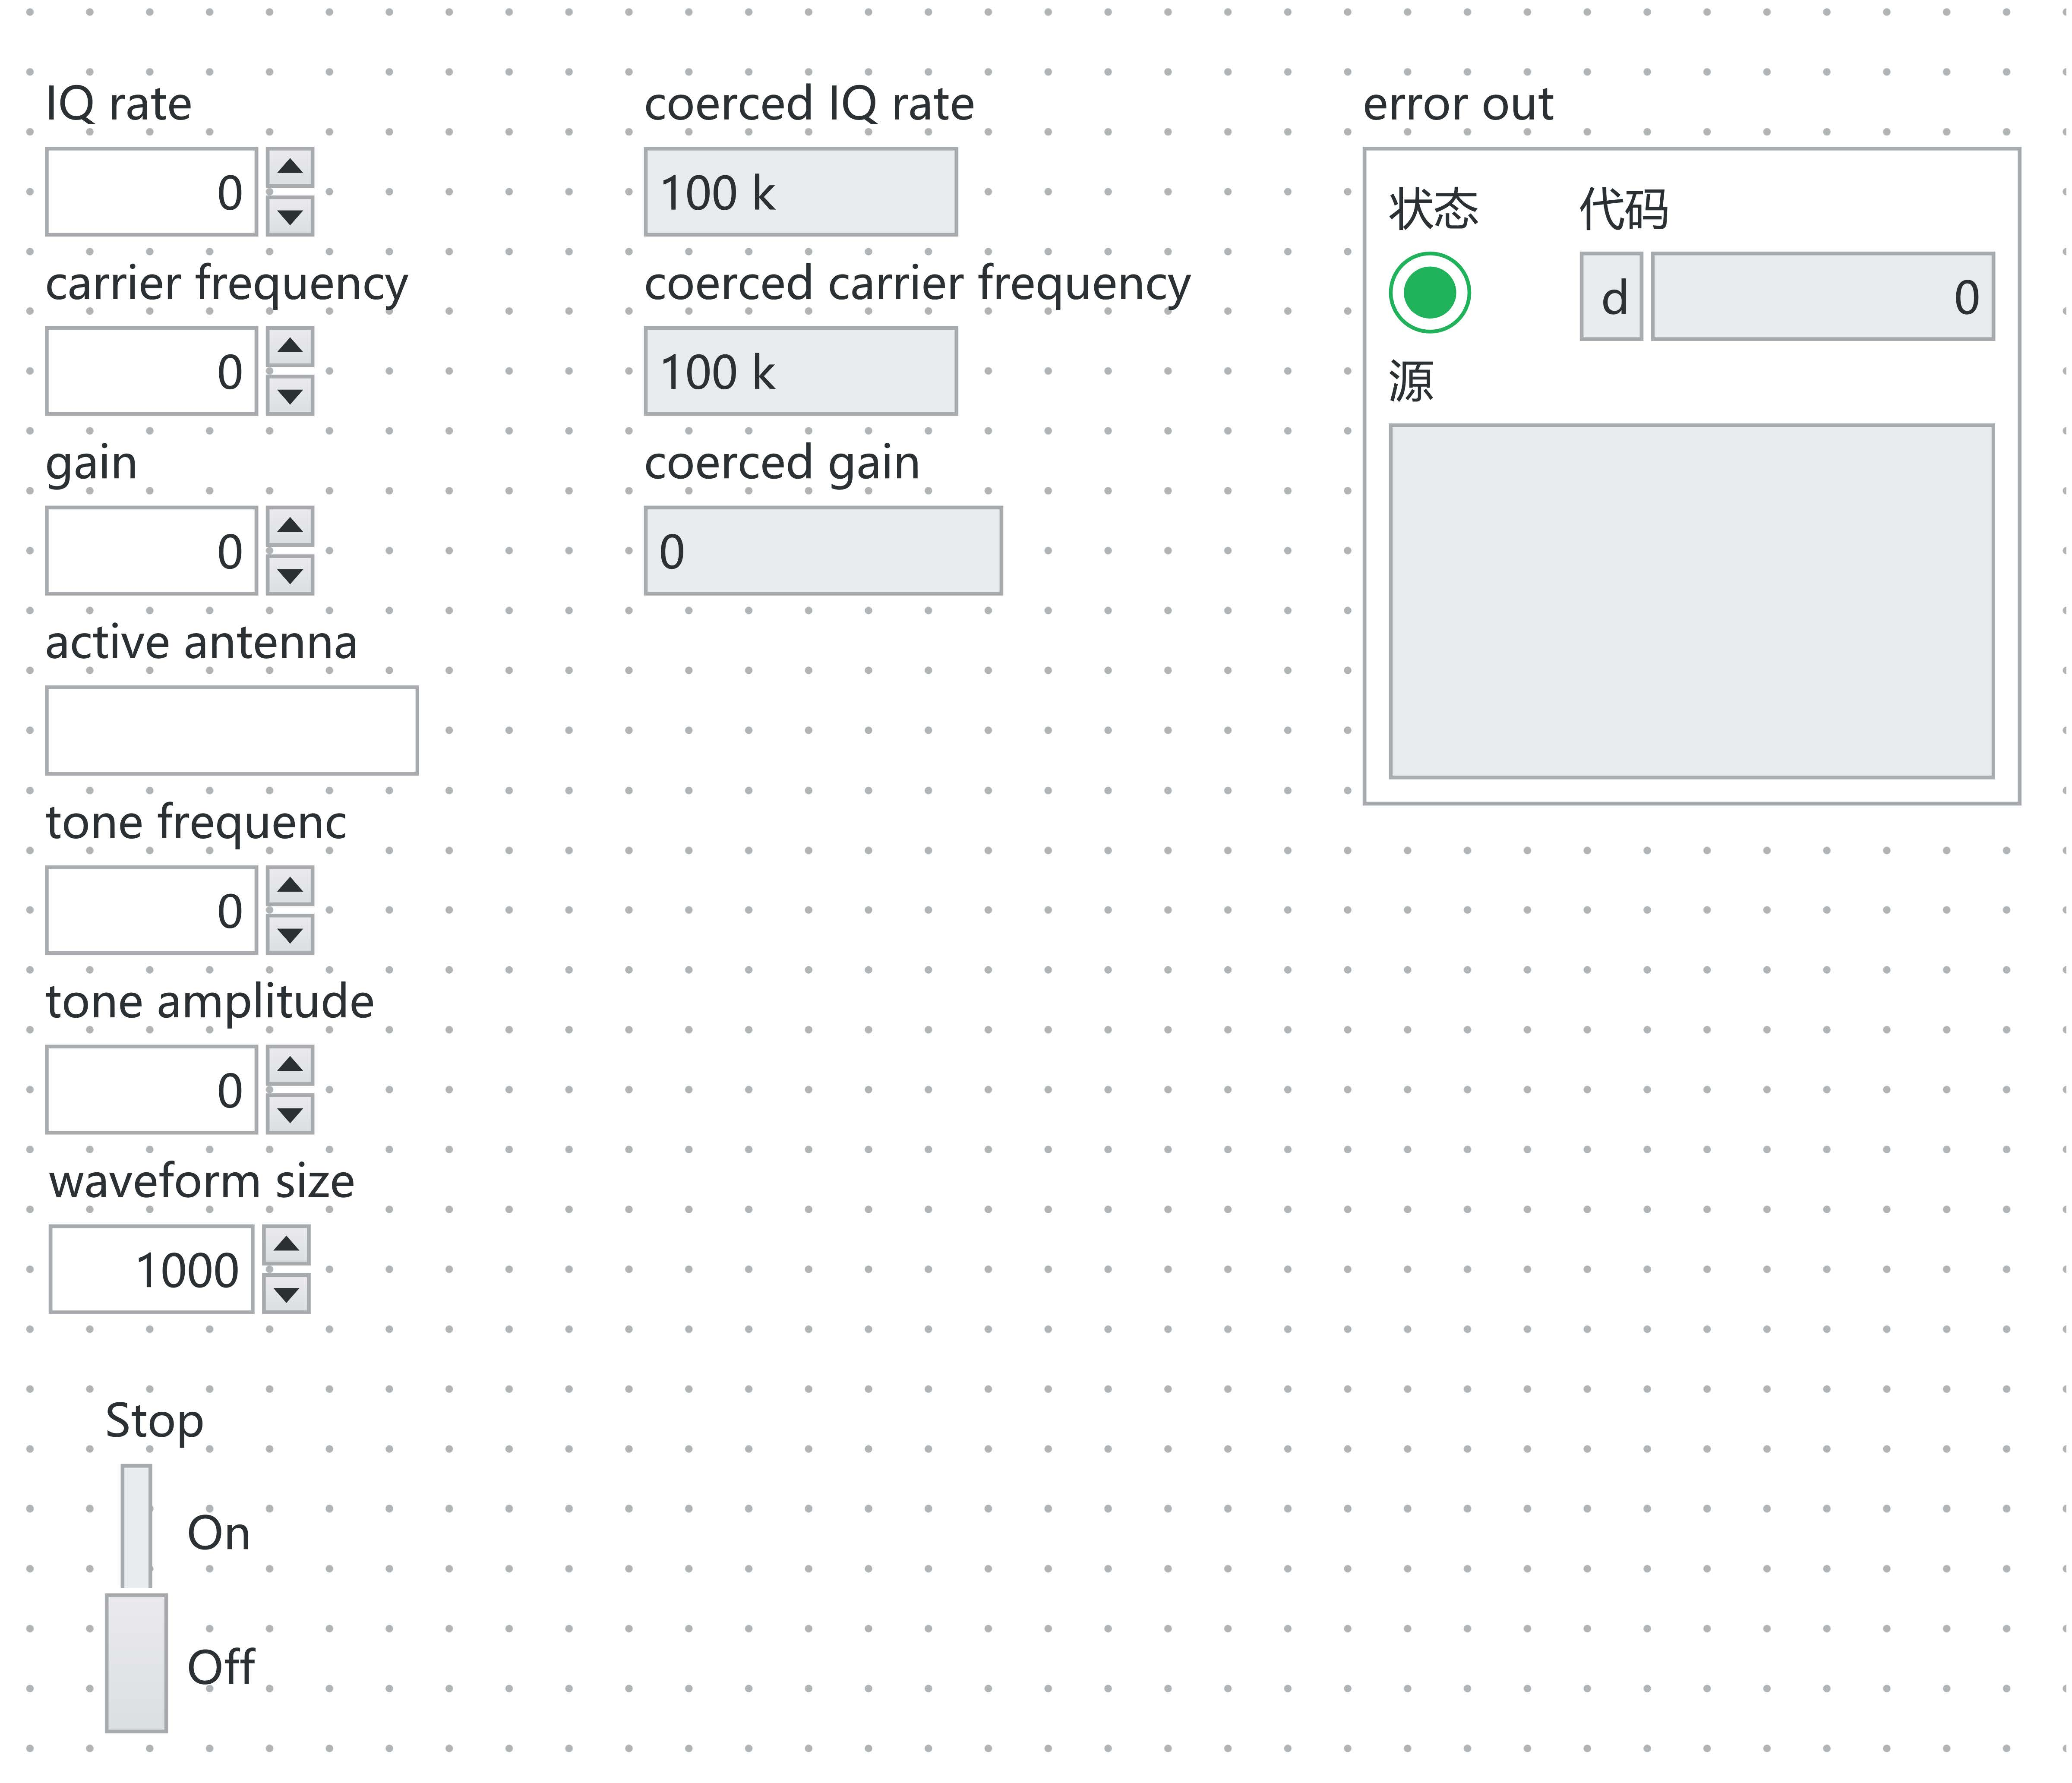
\includegraphics[width = 0.4\textwidth]{lab9/double-side_IQ-b.jpg}
    \caption{双边带调制前面板图}
\end{figure}

\begin{figure}[H]
    \centering
    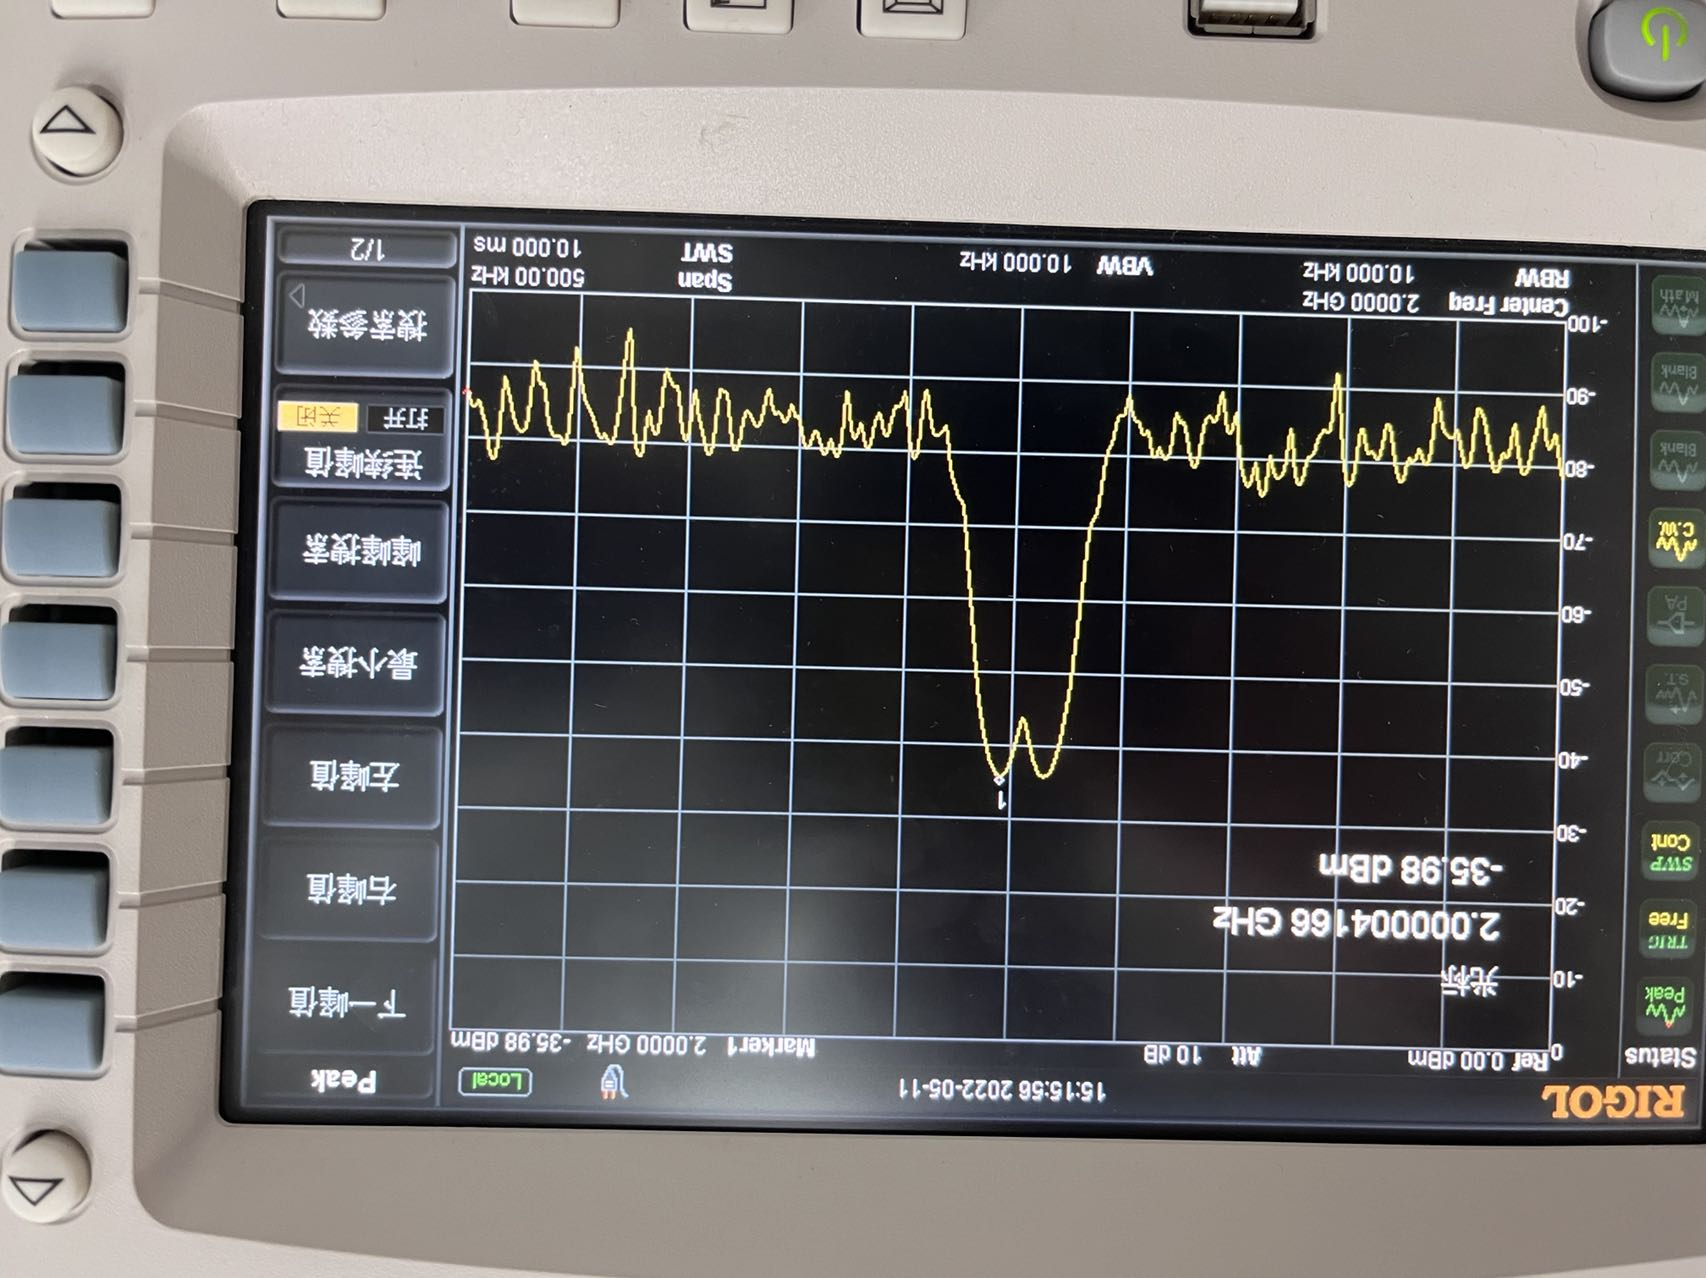
\includegraphics[width = 0.4\textwidth,angle=180]{lab9/7.jpg}
    \caption{双边带调制信号频谱图示例}
\end{figure}

\subsection{构建 USRP 接收器}
\begin{figure}[H]
    \centering
    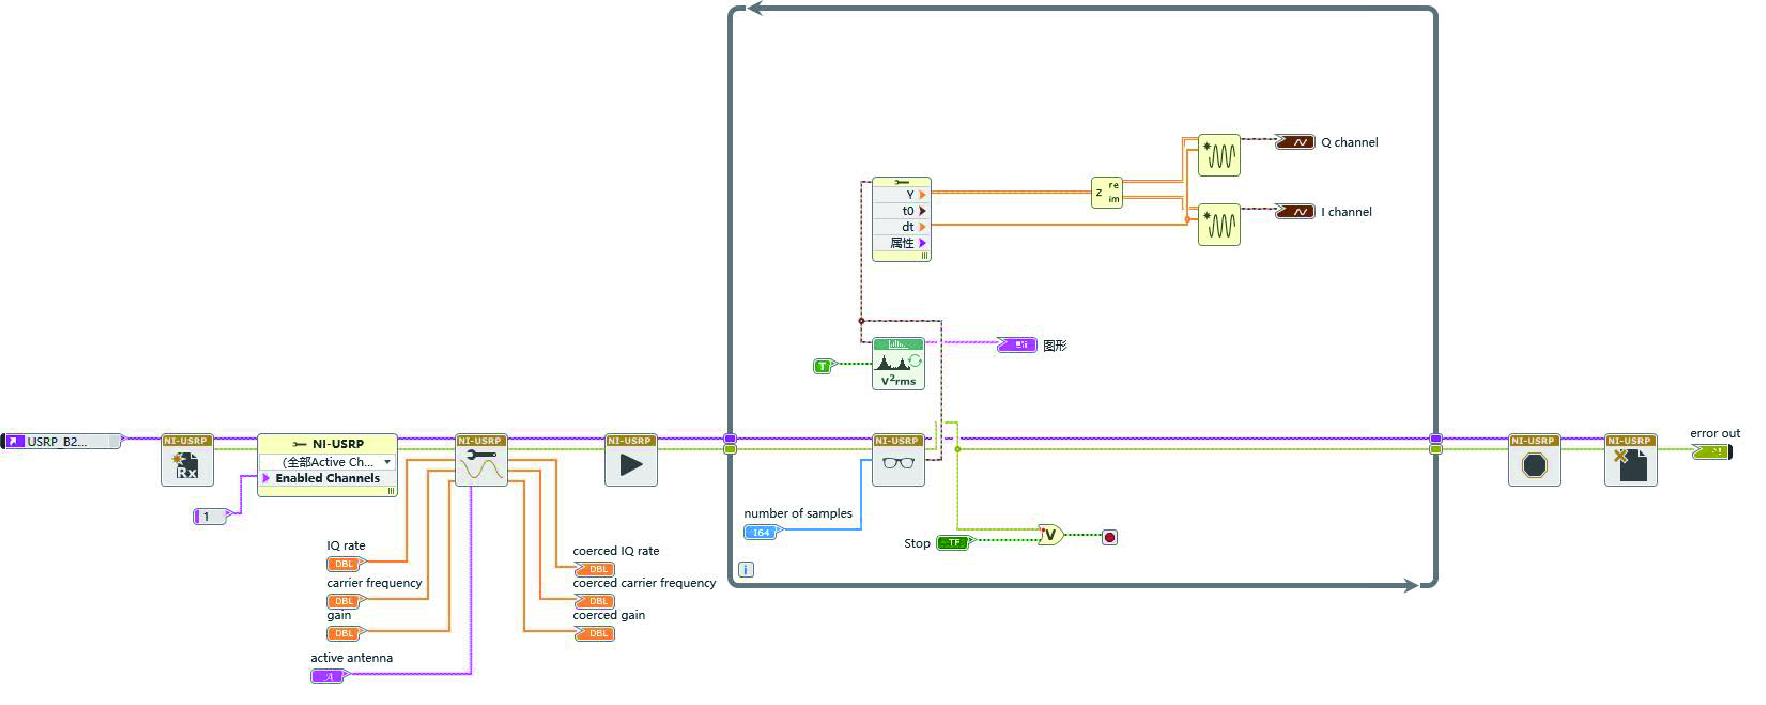
\includegraphics[width = 0.4\textwidth]{lab9/Rx-a.jpg}
    \caption{信号接收电路图}
\end{figure}
\begin{figure}[H]
    \centering
    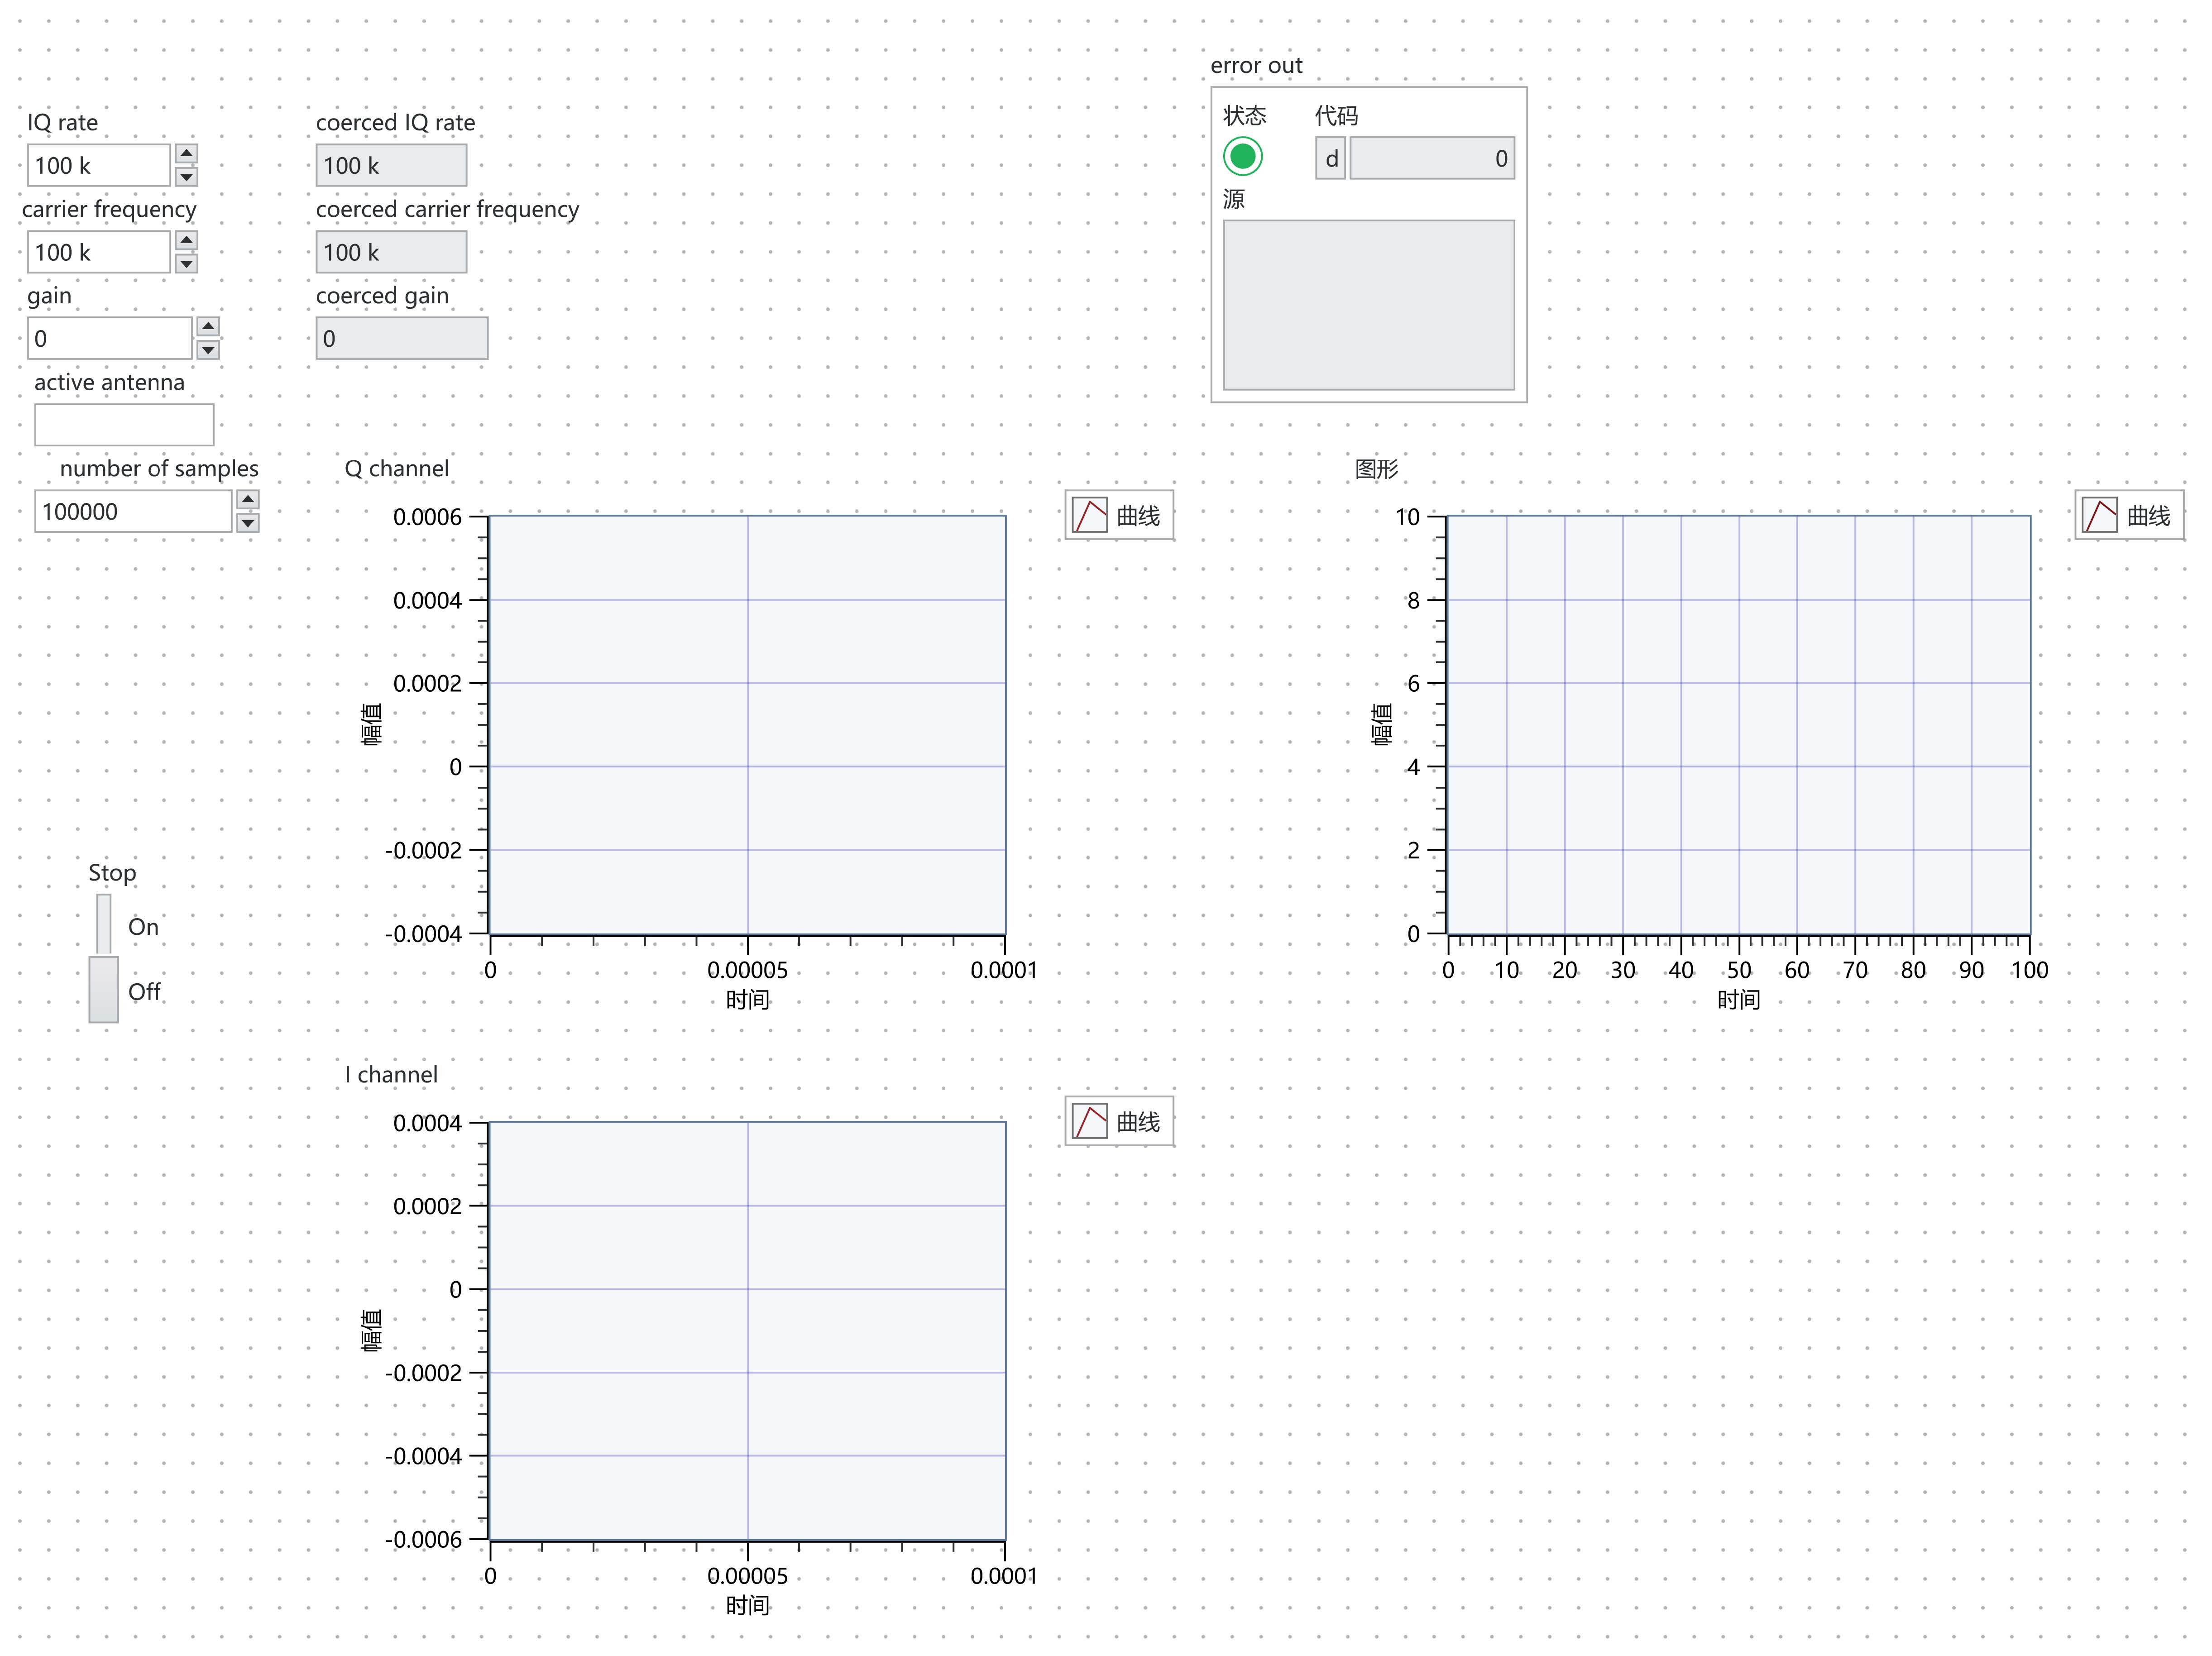
\includegraphics[width = 0.4\textwidth]{lab9/Rx-b.jpg}
    \caption{信号接收前面版图}
\end{figure}

设置好参数,运行电路,使用 SMA 电缆将 RF0 的 TX1 端口和 RF1 的 RX2 端口连接起 来。

\subsection{问题2}
(1) 先运行“upper-side\_IQ.gvi”,然后再运行“Rx.gvi”,观察接收信号的波形和 频谱
\begin{figure}[H]
    \centering
    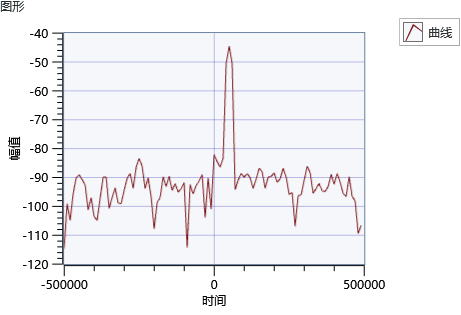
\includegraphics[width = 0.4\textwidth]{lab9/UPPER.png}
    \caption{信号接收频谱图}
\end{figure}
\begin{figure}[H]
    \centering
    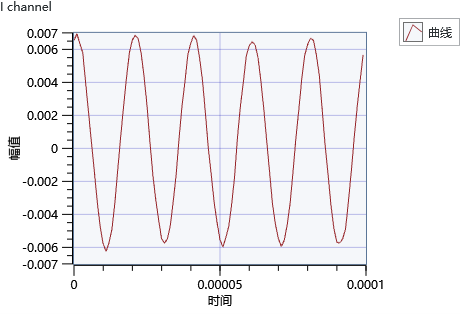
\includegraphics[width = 0.4\textwidth]{lab9/UPPER_I.png}
    \caption{接收到的I信号}
\end{figure}
\begin{figure}[H]
    \centering
    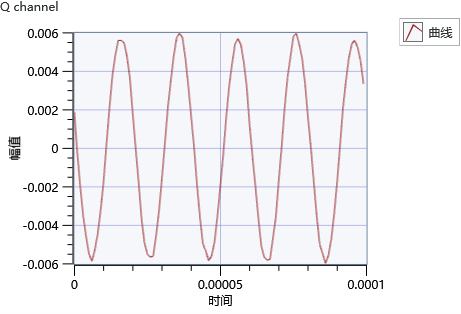
\includegraphics[width = 0.4\textwidth]{lab9/UPPER_Q.png}
    \caption{接收到的Q信号}
\end{figure}

(2) 分别运行“lower-side\_IQ.gvi”和“double-side\_IQ.gvi”的情况下,运行“Rx.gvi”, 观察接收信号的波形和频谱。

下边带信号:
\begin{figure}[H]
    \centering
    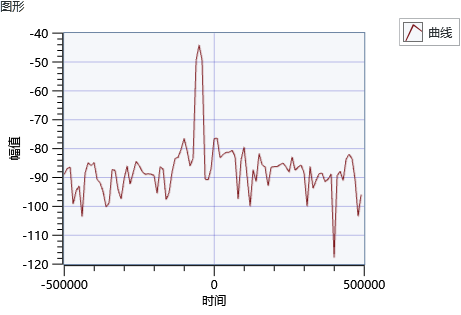
\includegraphics[width = 0.4\textwidth]{lab9/LOWER.png}
    \caption{下边带信号接收频谱图}
\end{figure}

双边带信号:

\begin{figure}[H]
    \centering
    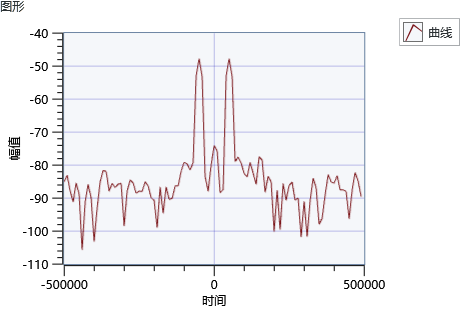
\includegraphics[width = 0.4\textwidth]{lab9/DOUBLE.png}
    \caption{双边带信号接收频谱图}
\end{figure}

(3) 在“lower-side\_IQ.gvi”中,将正弦波信号改为方波信号,观察接收信号频谱的 变化。
\begin{figure}[H]
    \centering
    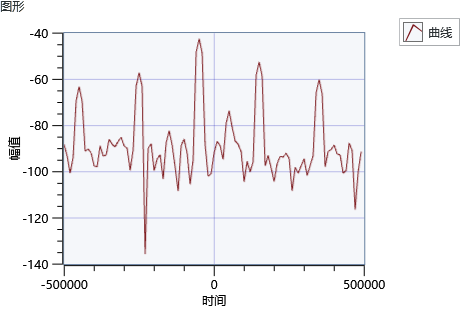
\includegraphics[width = 0.4\textwidth]{lab9/LOWER_SQUARE.png}
    \caption{信号接收频谱图}
\end{figure}
\begin{figure}[H]
    \centering
    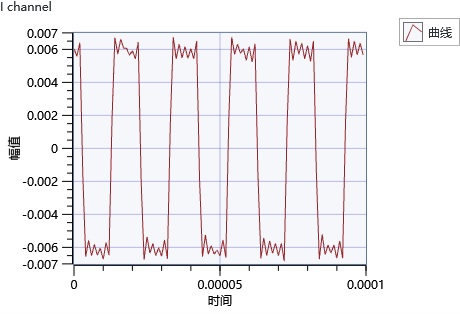
\includegraphics[width = 0.4\textwidth]{lab9/LOWER_SQUARE_I.png}
    \caption{接收到的I信号}
\end{figure}
\begin{figure}[H]
    \centering
    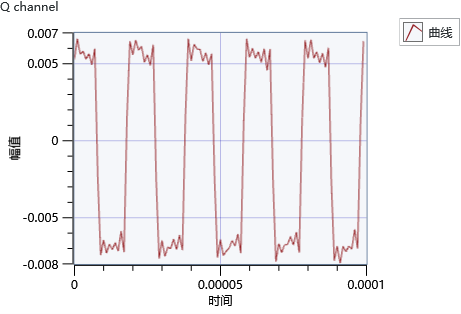
\includegraphics[width = 0.4\textwidth]{lab9/LOWER_SQUARE_Q.png}
    \caption{接收到的Q信号}
\end{figure}
\end{document}